\chapter{\textsc{Elektra}}
\label{chapter:approach}

\chapterprecishere{You never change things by fighting the existing reality. To change something, build a new model that makes the existing model obsolete.\par\raggedleft--- \textup{Buckminster Fuller}}
\chapterhung

In this chapter we formalize a model of \elektra{}'s central parts.
They capture the whole framework of \elektra{}.
We do not provide any rationale but explain internal dependences of the model.
We concisely describe all parts relevant for further development of this book, including the modular configuration specification language \elektra{Spec}.
In later chapters, we will present the rationale and the connection to the requirements.

In \secref{keyset} we discuss a common data structure all other parts of the framework \elektra{} relies on.
We use it to represent configuration settings and specifications for both in-memory access, code generation, and persistent configuration files.
We introduce a syntax suitable for this book to denote configuration settings and specifications.

In \secref{users-view} we explore the user's view of \elektra{}.
We elaborate on the fundamentals of the modular configuration specification language \elektra{Spec} and how \elektra{Spec} provides guarantees for users concerning configuration access.
We discuss how to facilitate the contextual classes that implement type-safe contextual values.

In \secref{kdb} we take the system's perspective.
We describe the essence of backends and the algorithms used by \elektra{Lib}.
We introduce how \elektra{Lib} keeps the in-memory data structure in sync with the execution environment.
We discuss the default behavior of the key database and how the behavior is redefined via \elektra{Spec}.

In \secref{api} we accustom us with the details of frontends.
We introduce another abstraction to transform configuration settings and specifications to source code.
Based on this abstraction, we show how \elektra{Gen} generates contextual classes and prove the absence of a run-time error concerning unavailable configuration settings.













\section{Data Structure}
\label{sec:keyset}
\label{sec:api-data-structure}

A key-value pair is the simplest generic data structure~\cite{strang2004context}.
While syntactically plenty of different configuration files are available, they all can be represented as key-value pairs as discussed in \secref{configuration-file-formats}.
In this section we define a key-value data structure suitable to contain configuration settings and specifications thereof.

\subsection{Preliminaries}

We start by defining the characters and strings needed to create key-value pairs:

\begin{definition}
The \intro{character set} $C$ includes all needed characters.
\label{def:comparison}
There is a total order on $C$ with the character slash ($\mlq/\mrq$) being the smallest character:
\[
	\forall x,y \in C: \mlq/\mrq \leq x \land (x \leq y \lor y \leq x) \land ((x \leq y \land y \leq x) \implies x=y)
\]
A \intro{string} $\overrightarrow{C}$ is a (possibly empty) sequence of characters in $C$.
A \intro{non-empty string} $\overrightarrow{C_{\geq1}}$ has a length of at least one.
A \intro{value} $\overrightarrow{C_\NullValue}$ is a string, that additionally can be $\NullValue$ (which is different from an empty string).
We call the set of all possible strings $\Strings$, the set of all possible non-empty strings \NonEmptyStrings, and the set of all possible values $\SetOfValues = \Strings \cup \{\NullValue\}$.
\end{definition}

We employ values $\in \SetOfValues$ as configuration values.
The value $\NullValue$ represents an available configuration value that intentionally was set to be not available.

We use the extended Backus--Naur form notation to specify syntax~\cite{wirth1977what,scowen1998extended,standard1996ebnf}.
We have two forms to denote nonterminals:
\begin{itemize}
\item
We write nonterminals in \synt{angles and italics}.
They are case-sensitive and either defined within grammars or in the surrounding text.
\item
We write nonterminals as symbols representing sets, such as $C$ and $\NonEmptyStrings$.
Here each element of the set is supposed to be in the specified syntax.
\end{itemize}
To avoid name collisions, some nonterminals defined within the grammar start with capitals.
We write terminals in \syntax{\lq^quotes and in typewriter^'}.
The quotes contain strings~$\in \Strings$ (or characters $\in C$, only in the next definition).
Furthermore, we write productions with \syntax{::=}, union with \syntax{|}, options with \syntax{[]}, groups for preferences with \syntax{()}, and any number of repetitions (including zero repetitions) in \syntax{\{\}}.

\begin{definition}
A \intro[white space]{white space} (in grammars denoted as \lq\WhiteSpace') is a character in $C$ to represent vertical space.
The set of \intro{special characters} $P \subset C$ is:

\begin{grammar}
\StashGrammar
<$P$> ::= \lq^/^' | \lq\texttt{\%}' | \lq^=^' | \lq^,^' | \lq^:^' | \lq\texttt{;}' | \lq\WhiteSpace' | \lq^[^' | \lq^]^'
\end{grammar}
\end{definition}

We denote a \intro[line break]{line break} in grammars as \lq\LineBreak', but assume for the discussion here that they are not considered as characters $\in C$ and thus cannot be part of strings or values.\footnote{
In the implementation special characters such as line breaks are escaped with complicated rules not relevant to the model.
We assume escaped line breaks to be characters different from \lq\LineBreak'.}

\begin{definition}
A \intro{clean string} $\CleanString$ is a sequence of non-special characters in $C \setminus P$, and $\overrightarrow{C_{\geq 1}'}$ is a non-empty sequence thereof.
We call the set of all possible clean strings $\CleanStrings$ and the set of all possible \intro[non-empty, clean string]{non-empty, clean strings} \NonEmptyCleanStrings.
We denote literal strings with \str{string} and string concatenation with $x \concat y$ ($x, y \in \Strings$).
\end{definition}

\begin{example}
The literal \str{example} is a string $\in \Strings$, a clean string $\in \CleanStrings$, and a non-empty, clean string $\in \NonEmptyCleanStrings$.
It is identical to the string \str{ex} $\concat$ \str{ample}.
The string \str{hello, world} is a string $\in \Strings$ but not a clean string, i.\,e., $\notin \CleanStrings$.
It contains two special characters: a comma and a white space (\lq\WhiteSpace').
\end{example}



\subsection{Key Names}
\label{sec:key-name}
\label{sec:key}


\begin{definition}
\label{def:basename}
\label{def:relative-key-name}
The set of \intro[relative key name]{relative key names} $\RelativeKeyNames$ is a subset of non-empty strings $\NonEmptyStrings$ according to the following grammar:
\begin{grammar}
<hierarchy level> ::= $\NonEmptyCleanStrings$ | \lq\texttt{\%}'

<basename> ::= <hierarchy level>

\let\sl\syntleft
\let\sr\syntright
\StashGrammar
<$\RelativeKeyNames$> ::= \{ <\sl hierarchy level>\sr \lq^/^' \} <\sl basename>\sr
\end{grammar}
\end{definition}

As shown in the grammar, a basename is a special case of a \intro{hierarchy level}:
We call the right-most hierarchy level \intro{basename}.
The meaning of the special characters in the relative key names are:

\begin{description}
\item[\lq\texttt{/}'] is the hierarchy separator, splitting up the relative key name into hierarchy levels.
\item[\lq\texttt{\%}'] denotes an empty hierarchy level.
\end{description}

\begin{example}
The string \lq\key{slapd/\%/bar}' is a relative key name.
Its hierarchy levels are \lq\key{slapd}', \lq\key{\%}', and \lq\key{bar}', where \lq\key{bar}' is additionally called basename.
\end{example}

\begin{definition}
\label{def:key-name}
The set of \intro[key name]{key names} $\KeyNames$ is defined by the following grammar, where each element in $\NameSpaces$ is a \intro{namespace}:

\begin{grammar}
\StashGrammar
<$\KeyNames$> ::= [ $\NameSpaces$ \lq^:^' ] \lq^/^' $\RelativeKeyNames$

<$\NameSpaces$> ::= \lq^spec^' | \lq^proc^' | \lq^dir^' | \lq^user^' | \lq^system^'
\end{grammar}
If a key name does not have the optional namespace and starts with \lq^/^', we say the key name has namespace $\EmptyNameSpace$ (which is not included in $\NameSpaces$).
\end{definition}

The elements of $\NameSpaces$ represent the namespaces \namespace{spec}, \namespace{proc}, \namespace{dir}, \namespace{user}, and \namespace{system}.
They have fixed semantics described in \secref{namespace}.

To avoid name collisions of key names we have two options:
\begin{itemize}
\item If we speak of the same configuration setting from different \empha[configuration source]{configuration sources}, we use namespaces.
The namespaces $\NameSpaces$ resolve conflicts between otherwise identical key names.
\item Otherwise, we introduce further hierarchy levels.
\end{itemize}

\begin{example}
The string \lq\key{user:/slapd/\%/bar}' is a key name.
Its hierarchy levels are the strings \lq\key{slapd}', \lq\key{\%}', and \lq\key{bar}', where the string \lq\key{bar}' is the basename.
The string \str{user} acts as its namespace \namespace{user}.
\end{example}

For simplicity and easier distinction with other strings, we leave out the \lq{}quotes' for (relative) key names.

\begin{example}
The string \key{/slapd} is a key name.
Its namespace is $\EmptyNameSpace$.
The only hierarchy level is also the basename, which is \key{slapd}.
\end{example}

We define the following operators on key names.
\begin{definition}
Using $x,y \in \KeyNames$ and $n \in \NameSpaces$:
\begin{align*}
x \leq y & \quad \text{is defined by lexicographical comparison of the characters.}  \\
\text{removeNamespace} (x) &=
\begin{dcases}
x \text{ if the namespace of } x \text{ is } \EmptyNameSpace \\
y \text{ otherwise, where  } x = n \concat \mlq{:}\mrq \concat y
\end{dcases}
\end{align*}
\end{definition}
\vspace{1em}

\begin{example}
For every $x \in C$, \key{user:/a/a} $\leq$ \key{user:/a}$x$\key{a} is true.
A further example of lexicographical comparison is given in \exref{order} on page \pageref{ex:order}.
\end{example}

\begin{example}
\emph{removeNamespace}(\key{user:/slapd/\%/bar}) gives \key{/slapd/\%/bar}.
\end{example}


\subsection{Keys and Key Sets}

\begin{definition}
The set of \intro[metakey!name]{metakey names} $M$ is a subset of the set of relative key names $\RelativeKeyNames$.
$G$ is a set of grammars.
The metafunction $\Psi$ is a global mapping from every defined metakey name $m \in M \subset \RelativeKeyNames$ to a grammar $g \in G$, i.\,e., $\Psi \colon M \mapsto G$.
$X_g \subseteq \Strings$ is the set of strings that forms the language described by $g \in G$.
\intro[metakey!value]{Metakey values} are elements of the set $\MetaKeyValues$.
\end{definition}

In the extensible meta-specification describing \elektra{Spec}, we define all grammars $g \in G$ for the metakey names $M$.
We give some of these grammars in the course of this chapter.
Users can extend $M$ but cannot redefine $\Psi$ for existing elements in $M$.
With every new element in $m \in M$, the user also needs to add a grammar $g \in G$ and add $(m, g) \in \Psi$.
Every extension automatically adds to the set $\MetaKeyValues$ because it is the set that includes all strings according to the languages described by all grammars in $G$.

\begin{example}
Given \synt{number} as decimal number, let us define \synt{property check/range} $\in G$ for \lq\texttt{check/range}' $\in M$ assigned by $\Psi(\property{check/range}\ \,)$:

\begin{grammar}
<property check/range> ::= <range> \{ \lq^,^' <range> \}

<range> ::= <number>  \textquoteleft^-^' <number>
        \alt <number>
\end{grammar}

Thus ^1,2,4,8,16^ as given in \exref{introduction-solution} on page \pageref{ex:introduction-solution} is a valid metakey value for \property{check/range}.
\end{example}

\begin{example}
\label{ex:types}
Let us define \synt{property type} $\in G$ for \lq\texttt{type}' $\in M$ assigned by $\Psi(\property{type})$:

\begin{grammar}
<property type> ::= \lq^boolean^' | \lq^string^' | \lq^short^' | \lq^unsigned_short^' \alt \lq^long^' | \lq^unsigned_long^' | \lq^long_long^' \alt \lq^unsigned_long_long^' | \lq^float^' \alt \lq^double^' | \lq^char^' | \lq^any^' | \lq^octet^'
\end{grammar}

Thus ^long^ as given in \exref{introduction-solution} is a valid metakey value for \property{type}.
\end{example}

\begin{definition}
A key is a record $\left<k, v, \mu\right>$ with the following fields:
\begin{description}
\item[$k$] is a key name from $\KeyNames$.
\item[$v$] is a value from $\SetOfValues$.
\item [$\mu$] is a function, defined as $\mu \colon M \mapsto \MetaKeyValues$, which maps from metakey names to metakey values.
The grammar of each metakey value is defined by: $\forall r \in M\colon \mu(r) \in X_{\Psi(r)}$.
\end{description}
We call the set of all keys $\Keys$.
\end{definition}

A key $x$ holds the configuration value $x.v$ for a configuration setting with the name $x.k$.
The function $x.\mu$ assigns \intro{metadata} to this configuration setting.
We write ^Key^ if we refer to the class implementing keys.

\begin{example}
\label{ex:key}
The key $x = \langle$\key{user:/slapd/threads/listener}, ^4^, $\{\texttt{check/}$\linebreak$\texttt{range} \mapsto 1,2,4,8,16 \}\rangle$ has the key name $x.k$ \key{user:/slapd/threads/listener},
the value $x.v$ which is ^4^,
and the metadata $x.\mu$ that maps the metakey name \key{check/range} to the metakey value ^1,2,4,8,^^16^.
\end{example}

\begin{example}
The key $x = \langle$\key{user:/slapd/threads/enabled}, ^1^, $\{\texttt{type} \mapsto$ \allowbreak $\texttt{boolean} \}\rangle$ has the configuration value $x.v = 1$, which represents true.
\end{example}

We define the following operators on keys:

\begin{definition}
We use $x, y \in \Keys$, and $n \in \NameSpaces$:
\begin{align*}
\phantom{juhuuuuu}             x = y & \quad \iff x.k=y.k \\
                            x \leq y & \quad \iff x.k \leq y.k \\
                  n \concatkey x = y & \quad \text{ where } y.k = n \concat \mlq{:}\mrq \concat \text{removeNamespace} (x.k)
\end{align*}
\end{definition}

\begin{example}
With $x$ from \exref{key}, applying ^system^ $\concatkey x$ yields the key $y$ with the key name $y.k =$ \key{system:/slapd/threads/listener}.
\end{example}

\begin{definition}
We say a key $x$ \intro[namespace!is of]{is of} the namespace $n$ iff $x.k$ has the namespace $n$.
A \intro[cascading key]{cascading key} is of the namespace $\EmptyNameSpace$.
\end{definition}

\begin{example}
The key $x = \langle$\key{/slapd}, $\NullValue$, $\{ \}\rangle$ is of the namespace $\EmptyNameSpace$ and thus is a cascading key.
\end{example}

If a configuration value represents a boolean, by convention, we use the string ^0^ to represent false, and ^1^ to represent true.

\begin{definition}
\label{def:property}
Iff the key $x$ is of the namespace \namespace{spec}, we call a metakey name also a \intro[property!name]{property name}, a metakey value also a \intro[property!value]{property value}, and the mapping $x.\mu$ also a \intro{property}.
\end{definition}

Property names define the syntax of property values via $\Psi$.

\begin{example}
The key $x = \langle$\key{spec:/slapd/threads/listener}, $\NullValue$, $\{\texttt{check/}$\linebreak$\texttt{range} \mapsto 1,2,4,8,16 \}\rangle$ has the (only) property name \property{check/range} with its property value \property{1,2,4,8,16}.
Thus the (only) property of $x$ is \property{check/range} $\mapsto 1,2,4,8,16$.
\end{example}



\begin{definition}
A key set $K \subseteq \Keys$ is a totally ordered set of keys where ordering is defined by $\leq$ on keys.
We call the set of all key sets $\KeySets$.
The key set without any key is called the \intro{empty key set} $\EmptyKeySet$.
The nullary operator $\NullKey$ returns a special key that indicates the absence of a key.
The key $\NullKey$ cannot be part of a key set.
The set with all keys including this special key is $\Keys_\NullKey = \Keys \cup \{\NullKey\}$.
\end{definition}

We write ^KeySet^ if we refer to the class implementing key sets.

\begin{figure}[htp]
\centering
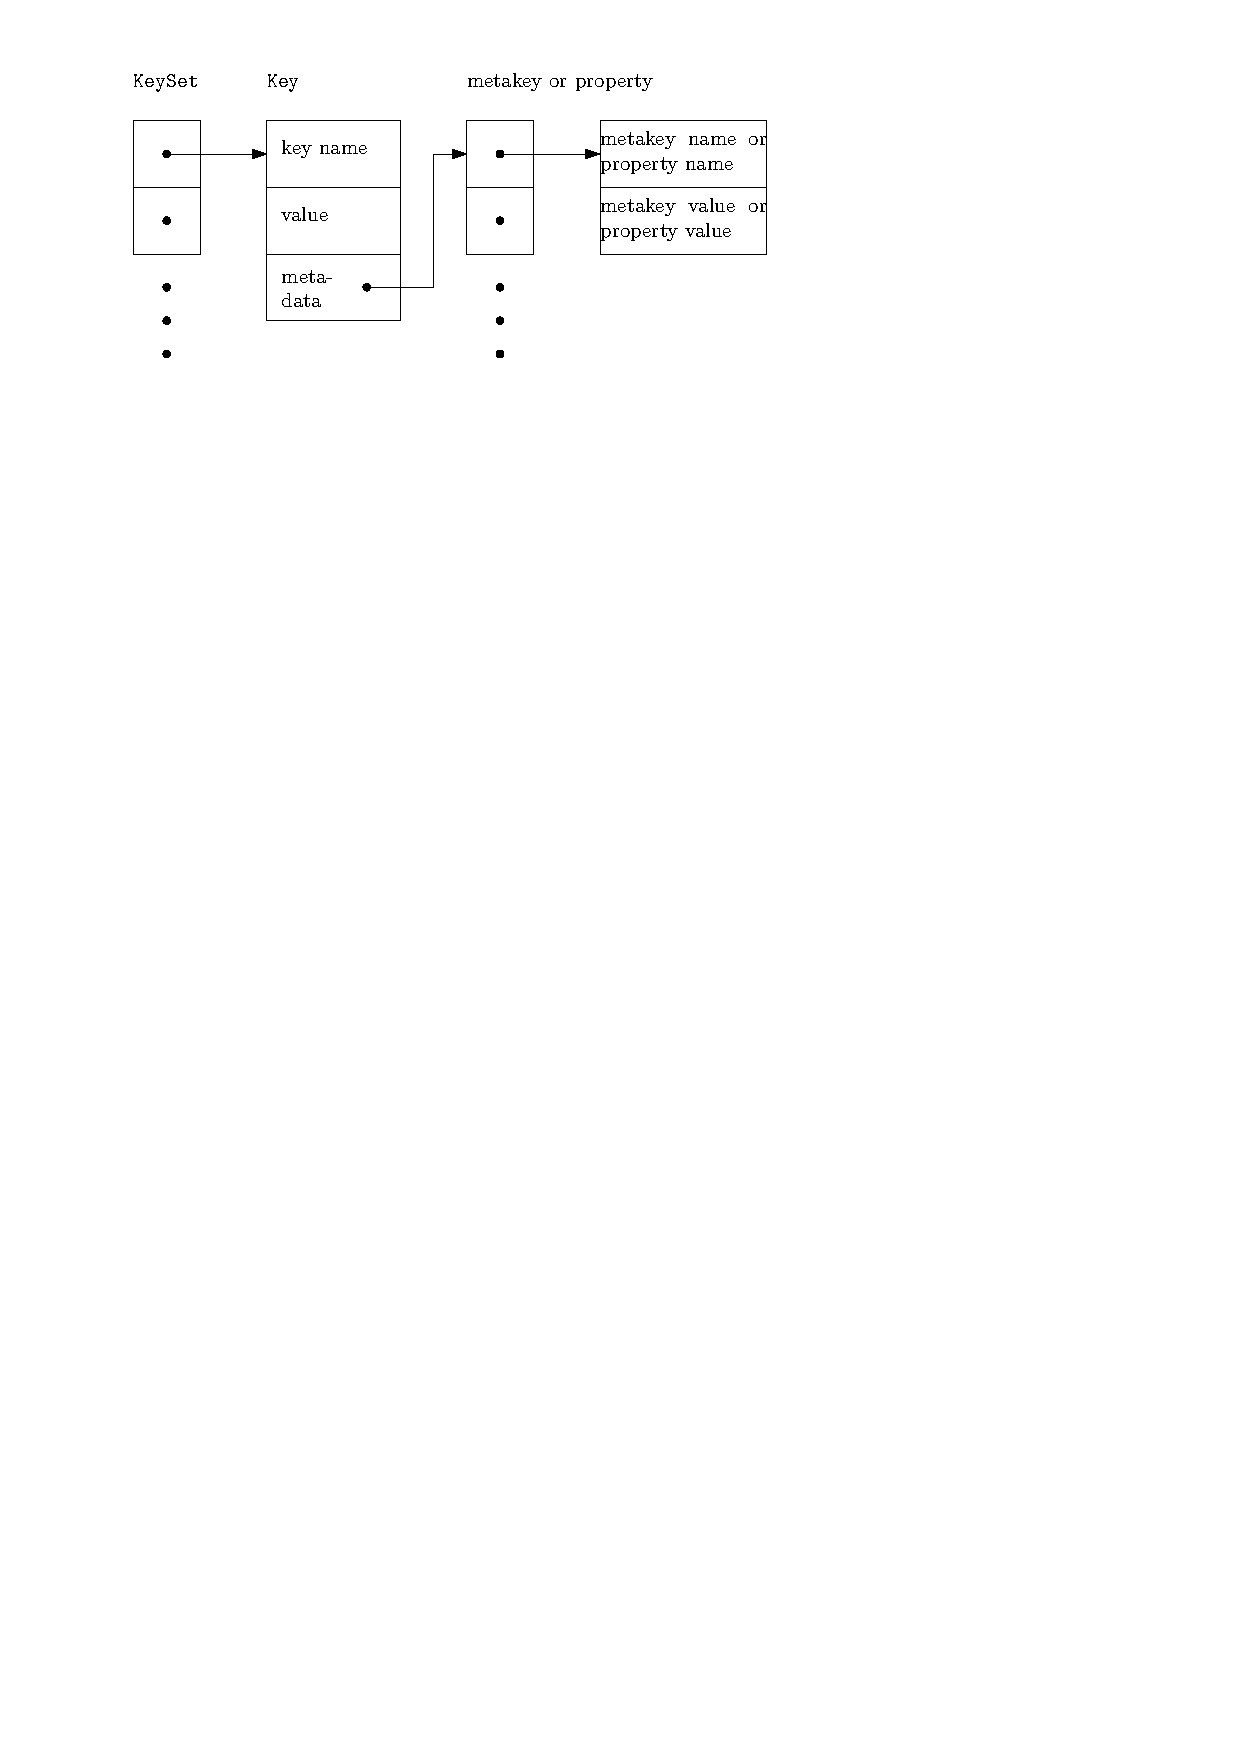
\includegraphics{keyset}
\caption{\texttt{KeySet}: \elektra{}'s data structure.}
\label{fig:keyset}
\end{figure}

A key set represents configuration settings and specifications.
\figref{keyset} gives us a visual representation of a key set.

In the next two sub-sections, we define the two most important operations on a key set.


\subsection{Appending}

Let us start with the definition of the ^ksAppend^ operation for $K$.

\begin{definition}
We use $x, y \in \Keys$ and $s \in \KeySets$:
\begin{align*}
\phantom{holahola}
ksAppend(s, x) =
\begin{dcases}
s \cup \{ x \}                     & \text{ if } \forall y \in s : y.k \neq x.k \\
(s \setminus \{ y \}) \cup \{ x \} & \text{ if } y \in s,\ y.k = x.k
\end{dcases}
\end{align*}
\end{definition}

The result of the function ^ksAppend^ is a key set that has the key $x$ appended to the key set $s$.
If a key with the key name $x.k$ is already present, it will be replaced by the key $x$.
Key sets are exclusively constructed as follows:
We start with the empty key set $\EmptyKeySet$ and repeatedly append keys to it using ^ksAppend^.

\begin{example}
After applying $\texttt{ksAppend} (\texttt{ksAppend} (\EmptyKeySet, \langle$\key{user:/x}, ^foo^, $\{ \}\rangle), \langle$\key{user:}\linebreak\key{/x}, ^bar^, $\{ \}\rangle)$, we have constructed the key set $\{ \langle$\key{user:/x}, ^bar^, $\{ \}\rangle \}$.
\end{example}

\begin{lemma}
If a key set is constructed by repeatedly applying ^ksAppend^ to the initially empty key set, then keys within the constructed key set are unique with respect to their key name $k$.
Given the natural numbers $n, m, b$ (including $0$), the keys $x_1, \ldots x_n \in \Keys$, and the key set $s \in \KeySets$, where $s$ was constructed using $\texttt{ksAppend} (\ldots \texttt{ksAppend} (\EmptyKeySet, x_1)  \ldots, x_n)$ the following statement $A(n)$ is always true:
\begin{equation}
\forall x_m, x_b \in s : x_m \neq x_b \implies x_m.k \neq x_b.k
\end{equation}
\vspace{-2em}
\end{lemma}

\begin{proof}
\begin{description}[font=\textit]
\item[Base case:] The only possible way to construct a key set is by subsequent use of ^ksAppend^.
Given the key $x_1 \in \Keys$ the induction start must be $\texttt{ksAppend} (\EmptyKeySet, x_1)$.
Trivially, $x_1.k$ is unique in a key set only containing $x_1$, i.\,e., $A(1)$ always holds.
\item[Induction step:] Suppose the hypothesis---that $A(n)$ is true---holds for the appended keys $x_1, \ldots x_n \in \Keys$, we have to show that $A(n) \implies A(n+1)$ holds for all $n$.
The proof---that adding a key $x$ to $s$ cannot change the uniqueness of $x.k$---directly follows from the definition of ^ksAppend^:
\begin{itemize}
\item If $x.k$ is already present as key name in $s$, then appending $x$ causes the removal of the key that has the key name $x.k$.
Therefore, no key with the same key name is present.
\item If $x.k$ is not present in $s$, $x$ is added to s and is the unique entry with the key name $x.k$.
\end{itemize}
\end{description}
\end{proof}


\subsection{Lookup}
\label{sec:approach-lookup}

Let us define the ^ksLookup^ operation on $K$.

\begin{definition}
We use $l \in \Keys$, $z \in \Keys_\NullKey$, and $c \in \KeySets$.
\texttt{ksLookup}$(c, l) = z$ searches the key $l$ in the key set $c$ and returns $z \in (c \cup \{\NullKey\})$.
The key $l$ is the key to be looked up.
^ksLookup^ has the signature $\KeySets \times \Keys \to \Keys_\NullKey$.
The nullary operator $\NullKey$ represents the not-found key.
Iff the key was found, ^ksLookup^ returns a key from $c$.
\end{definition}

The algorithm ^ksLookup^ provides two different views on a key set:
\begin{enumerate}
\item If $l$ is of namespace $\EmptyNameSpace$, a \intro{cascading lookup} is used.
A cascading lookup consists of the following steps:
\begin{enumerate}
\item
The function ^ksLookup^ can be extended.
Such extensions allow us to consider more keys to improve context awareness and to visualize the lookup process.
If an extension is available, the cascading lookup tries to look up the key $l$ with the lookup logic as provided by the extension.
We present an extension ^lookupByExtension^ later in \secref{approach-context-aware-lookup}.
\item
The namespace \namespace{spec} is considered.
If the key ^spec^ $\concatkey l$ is found, we evaluate its properties.
We show the algorithm ^lookupBySpec^ in \secref{lookup-by-spec}.

\item
Otherwise, as shown in \figref{cascading}, we return a key with one of the following key names:
^proc^ $\concatkey l$, ^dir^ $\concatkey l$, ^user^ $\concatkey l$, and ^system^ $\concatkey l$ (in this preference).
\end{enumerate}

\begin{figure}[htp]
\centering
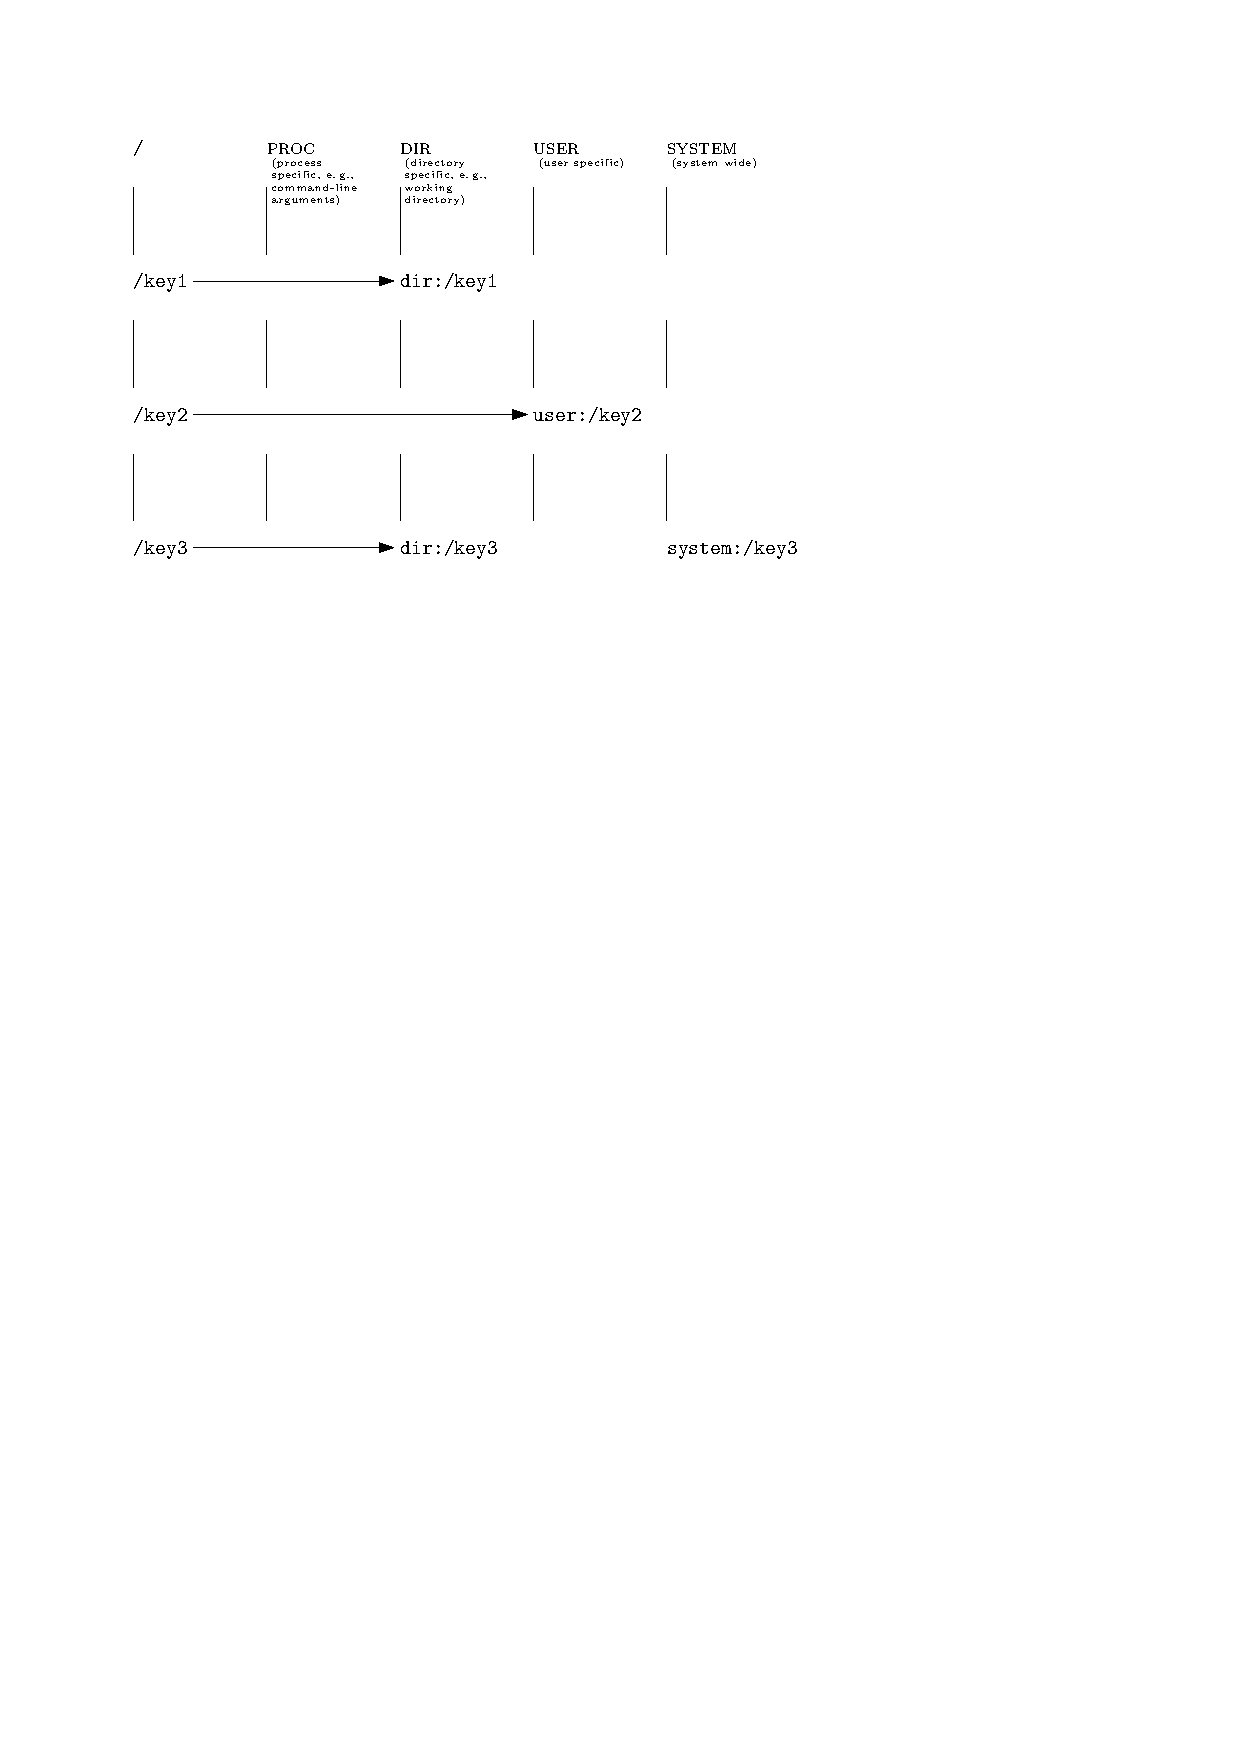
\includegraphics{cascading}
\caption[Cascading Lookup.]{Cascading lookup in \elektra{}.
Arrows indicate the lookup procedure if calling \texttt{ksLookup} with \texttt{/key1} to \texttt{/key3}.
The arrow ends at the key which is returned.
The key \texttt{system:/key3} is not found.
Explanations about namespaces follow later.
}
\label{fig:cascading}
\end{figure}

\item If the lookup key $l$ is not of namespace $\EmptyNameSpace$, ^ksLookup^ guarantees for every return value $x$ that $x.k = l.k \iff x \neq \NullKey$.
I.\,e. ^ksLookup^ either returns a key with exactly the same key name or $\NullKey$.
This form of ^ksLookup^ is the non-cascading lookup.%
{\parfillskip=0pt \emergencystretch=.5\textwidth \par}
\end{enumerate}

\begin{lemma}
\label{lem:append}
Given any key set $s \in \KeySets$ and the key $k \in \Keys$, where $k$ is not of namespace $\EmptyNameSpace$, the following statement is always true:
\begin{equation}
\forall s,k : \texttt{ksLookup}(\texttt{ksAppend}(s, k), k) = k
\vspace{-1em}
\end{equation}
\end{lemma}

The proof of Lemma~\ref{lem:append} directly follows from the above definition of ^ksLookup^ and ^ksAppend^:
we know that $k$ gets appended to $s$, and because $k.k$ has a namespace it is found by $ksLookup$.


We influence the behavior of ^ksLookup^ by adding keys of the form ^spec^ $\concatkey l$ to the key set.
This way, we enable the system administrator to specify guarantees for a cascading lookup by modification of persistent keys' properties in the namespace \namespace{spec}.

For cascading lookups, it is possible that ^ksLookup^ finds the same key $x$ for different arguments of ^ksLookup^.
The function ^ksLookup^ with cascading lookups is no longer bijective, we only have the properties of a surjective function.
Because the key name of the parameter $l$ and the result $z$ can be different, it is important that the key name is part of the key:
From the returned key, we know the key name of the found key.

The cascading lookup is an important abstraction and applications exclusively rely on cascading lookups to look up their configuration settings.
Thus for applications, \intro[configuration setting]{configuration settings} are represented by a key set only considering the key names and configuration values returned from cascading lookups.
Only tools intended for system administrators use the non-cascading lookup, so that all keys can be administered.
\intro[configuration specification]{Configuration specifications} are written in \elektra{Spec} and are represented by a key set only considering the key names of the namespace \namespace{spec} and the key's properties.%
{\parfillskip=0pt \emergencystretch=.5\textwidth \par}



\subsection{Syntax}
\label{sec:syntax}

\begin{figure}[htp]
\centering
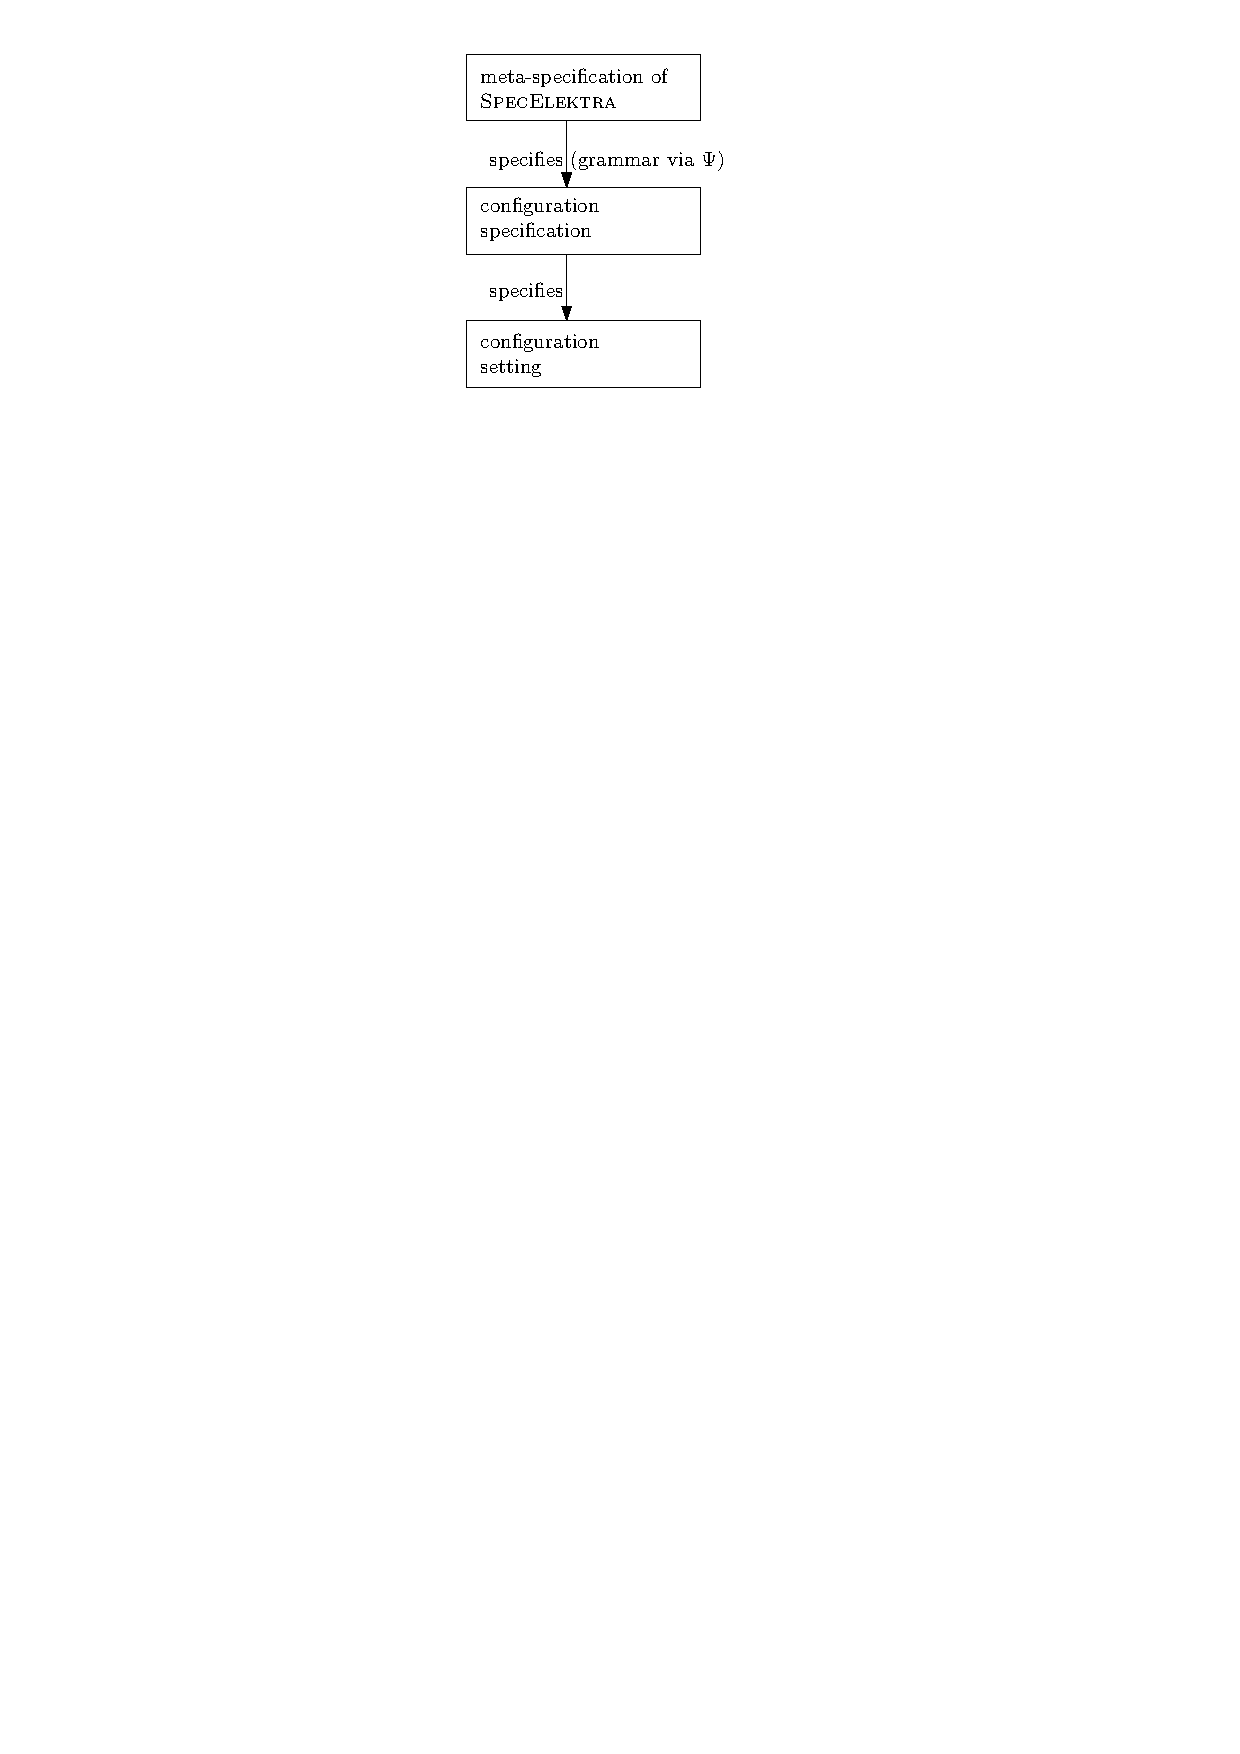
\includegraphics{metalevels}
\caption{Metalevels in \elektra{}.}
\label{fig:metalevels}
\end{figure}

As we see in \figref{metalevels}, three meta-levels of \elektra{} are important.
For the three meta-levels, we describe two syntaxes to denote a key set to be used in this book:
\begin{enumerate}
\item
Meta-specifications consist of a grammar $g \in G$ assigned by $\Psi$.
We explain the semantics mostly informally.
We do not need a special syntax for these specifications.
\item
For configuration specifications we need a way to denote key names and properties, but we do not need to include configuration values.
The grammar for this syntax will be given below.
\item
For configuration settings we only need to denote key names and configuration values without any support for metadata.
The grammar for this syntax will be given further below.
\end{enumerate}
The separation of syntax between configuration settings and specifications is purely for practical purposes so that different meta-levels are clearly distinguishable.
The distinction between configuration settings and specifications happens via namespaces and not via syntax:%
{\parfillskip=0pt plus .7\textwidth \emergencystretch=.5\textwidth \par}
\begin{itemize}
\item
If a key is in the namespace \namespace{spec}, the metadata is used as properties and the key represents a configuration specification.
\item
If a key is in another namespace, the metadata only describes the key itself, but does not specify the configuration setting.
Here the configuration value is the essential information.
Such keys are configuration settings.
\end{itemize}

For this book, we could have used every configuration file format that has a correspondence to a key set, for example, in XML syntax with metadata written as attributes.
We use, however, a simple INI-like syntax to illustrate key sets.
We exclusively rely on relative key names.

\subsubsection{Configuration Specifications}
\label{sec:syntax-spec}


Here we describe a syntax for configuration specifications.
They are used to specify configuration settings and configuration access in \elektra{Spec}.
A syntax usable for \elektra{Spec} needs to include relative key names (called $\RelativeKeyNames$, see \defref{relative-key-name}) with properties (see \defref{property}):

\begin{grammar}
<configuration specifications> ::= \{ <configuration specification>  \{ \lq\LineBreak' \} \}

<configuration specification> ::= \lq^[^' $\RelativeKeyNames$ \lq^]^' \lq\LineBreak' <properties>

<properties> ::= \{ <property> \lq\LineBreak' \}

<property> ::= \{  \lq\WhiteSpace' \}  <property name> \lq^:=^' [ <property value> ]
\end{grammar}

The absence of the \synt{property value} means that the property value is empty.
The grammar of the \synt{property value} is depending on its associated property name $x$.
The meta-specification specifies its grammar to be $\Psi(x)$.

\begin{example}
This is a configuration specification:

\begin{code}
[slapd/threads/listener]
  property1:=propvalue1
  property2:=propvalue2
\end{code}

In the first line, we write a relative key name within ^[]^.
\empha[property!value]{Property values} are assigned with ^:=^ to \empha[property!name]{property names}.
Every key can be specified with several properties.
The key with the key name ending with ^slapd/threads/listener^ has two properties as shown in lines 2 and 3.
The property name is ^property^$N$ and property value is ^propvalue^$N$.
The string ^propvalue^$N$ has a syntax according to $\Psi$(^property^$N$).
\end{example}




\subsubsection{Configuration Settings}
\label{sec:syntax-settings}

For configuration settings we do not necessarily need metadata nor properties.
We use the following grammar for configuration settings:

\begin{grammar}
<configuration settings> ::= \{ <configuration setting> \{ \lq\LineBreak' \} \} <configuration setting>

<configuration setting> ::= <relative key name> \Big[ \lq\lstinline[language=CfgElektra]^=^' [ <value> ] \Big] [ <comment> ]

<comment> ::=  \{ \lq\WhiteSpace' \} \lq^;^' $\Strings$
\end{grammar}

Absence of \synt{value} means that the value is an empty string and the absence of both \lq\lstinline[language=CfgElektra]^=^' and \synt{value} means that the value is $\NullValue$.
Assignment with \lstinline[language=CfgElektra]^=^, as opposed to ^:=^, is reserved for key-value pairs denoting configuration settings in configuration files.
This way, it is apparent for the reader that we are in a different meta-level and talking about concrete settings for applications.
For this book, we assume that the values do not have trailing spaces nor red semicolons \lq^;^'.

\begin{example}
By the use of the grammar above, we can specify configuration settings:

\begin{code}[language=CfgElektra]
slapd/threads/listener=1
slapd/key=1 ; comment
slapd
\end{code}

In the first line, we define that the key, identified with the relative key name \key{slapd/threads/listener}, has the configuration value ^1^.
The second line does the same with the key name ending with \key{slapd/key} but with a comment \lq{}{\color{purple}\texttt{ comment}}'.
In the third line, we define the key name ending with \key{slapd} to have the value $\NullValue$.
\end{example}

\subsection{Sort Order and Hierarchy}
\label{sec:approach-sort-order}

\begin{definition}
We say a key $x$ is \intro{below} a key $y$ iff the key name of $x$ has the key name of $y$ as prefix separated with a slash:
\begin{align*}
\texttt{below}(x, y) =
\begin{dcases}
&\top \text{ if } \exists s \in \RelativeKeyNames \colon x.k = y.k \concat \mlq\!/\mrq\! \concat s \\
&\bot \text{ otherwise}
\end{dcases}
\end{align*}
\vspace{.3em}\enlargethispage{2em}
\end{definition}


\begin{example}
The function \texttt{below}($\langle$\lq\key{user:/slapd/threads/listener}'$, \NullValue, \{ \}\rangle$,\linebreak $\langle$\lq\key{user:/slapd/threads}'$, \NullValue, \{ \}\rangle$) returns $\top$.
The function \texttt{below}($\langle$\lq\key{user:/slapd/threads/listener}'$, \NullValue, \{ \}\rangle$, $\langle$\lq\key{user:/slapd/key}'    $, \NullValue, \{ \}\rangle$) returns $\bot$.
\end{example}


\begin{definition}
A \intro{subtree} of a key $x$ and a key set $t$ is the key set $s$, which contains all keys in $t$ below $x$, as well as $x$.
We call $x$ the \intro{root} of the subtree.
\begin{equation}
\label{eq:subtree}
s = \{y \in t \mid below(x, y) \lor x=y \}
\end{equation}
\end{definition}

According to \defref{comparison}, we treat the special character ^/^ for the lexicographical comparison of keys with $\leq$ differently:
It is ranked first in the order of the character's precedence.\footnote{The implementation is efficient by separately storing key names modified in a way so that they are correctly compared with \texttt{memcmp}.}
Because of the special handling of ^/^, keys not within a subtree occur after keys within the same subtree.

\begin{example}
\label{ex:order}
Given the following key names:
\par
\begin{code}[language=CfgElektra]
a
a/a
a/b
a!a
\end{code}

Here ^a/a^ and ^a/b^ are below ^a^.
These three keys form a subtree with ^a^ as root.
The pure ASCIIbetical sort order\footnote{Sort by string comparison, i.\,e., the ASCII value of the characters.} would put ^a!a^ in the middle after ^a^.
Our chosen sort order allows us to efficiently operate on a hierarchy, for example, to cut out a subtree.
We look up the key ^a^, and keys below it (with respect to the hierarchy), are guaranteed to be subsequent, if there are any keys below ^a^.
\end{example}

\label{ex:array}
For iterating configuration settings, in most cases, the sort order of keys---within the same hierarchy level---is irrelevant.
If the order is important, we do not merely rely on how the key was inserted in the key set.
Instead the sort order is clearly visible within the key name.
We use a so-called \intro[array index]{array index} to indicate the order between otherwise identical key names or metakey names.
Such array indexes are also used if we have several key names for the same configuration setting.
We use the following convention for array indexes:%
{\parfillskip=0pt \emergencystretch=.5\textwidth \par}

\begin{enumerate}
\item The first array index is \lq^#0^'.
\item For the next array index, we increase the numerical part by incrementing it.
If the number of digits is increased by one, we add an underscore (\lq^_^') between \lq^#^' and the digits.
\end{enumerate}

While the algorithm keeps the key set ordered by the array index with any radix, for example, hexadecimal with the characters \verb+[A-F]+, we chose the decimal system.
It is trivial to know the quantity of \lq^_^' for any number by counting the digits and decrement the result.
With this convention we generate array indexes in a compact syntax, readable and writable by humans, while still using the sort order of decimals representing the array index.
Given \synt{number} as decimal natural number $\geq 0$, the grammar is:
\begin{grammar}
<array index> ::= \lq^#^' \{ \lq^_^' \} <number>
\end{grammar}

\begin{example}
The array index $1$ is written down as \lq^#1^', $10$ is written down as \lq^#_10^', $100$ is written down as \lq^#__100^'.
The sort order of these key names is:
\par
\begin{code}[language=CfgElektra]
#1
#_10
#__100
\end{code}
\phantom{}
\end{example}

\phantom{}

\begin{example}
To sort the key names ending with \key{a}, \key{b} and \key{c} in reverse order, we would use the following key names with array index from $0$ to $2$:
\par
\begin{code}[language=CfgElektra]
#0/c
#1/b
#2/a
\end{code}
\phantom{}
\end{example}























\section{User's View}
\label{sec:users-view}

Both system administrators and developers are users of \elektra{}.
In this section we consider these users together and frame \elektra{} with a focus of context-aware configuration from their point of view.
As shown in \figref{framework}, their main interactions with \elektra{} is by using frontends and \elektra{Spec}.
In this section we describe:
\begin{itemize}
\item How users get and set configuration settings and specifications (i.\,e., including specifications written in \elektra{Spec}).
\item How users map configuration files into a unified view for all applications.
\item How users share configuration settings.
\item How users enable context-aware configuration.
\end{itemize}

\begin{figure}[htp]
\centering
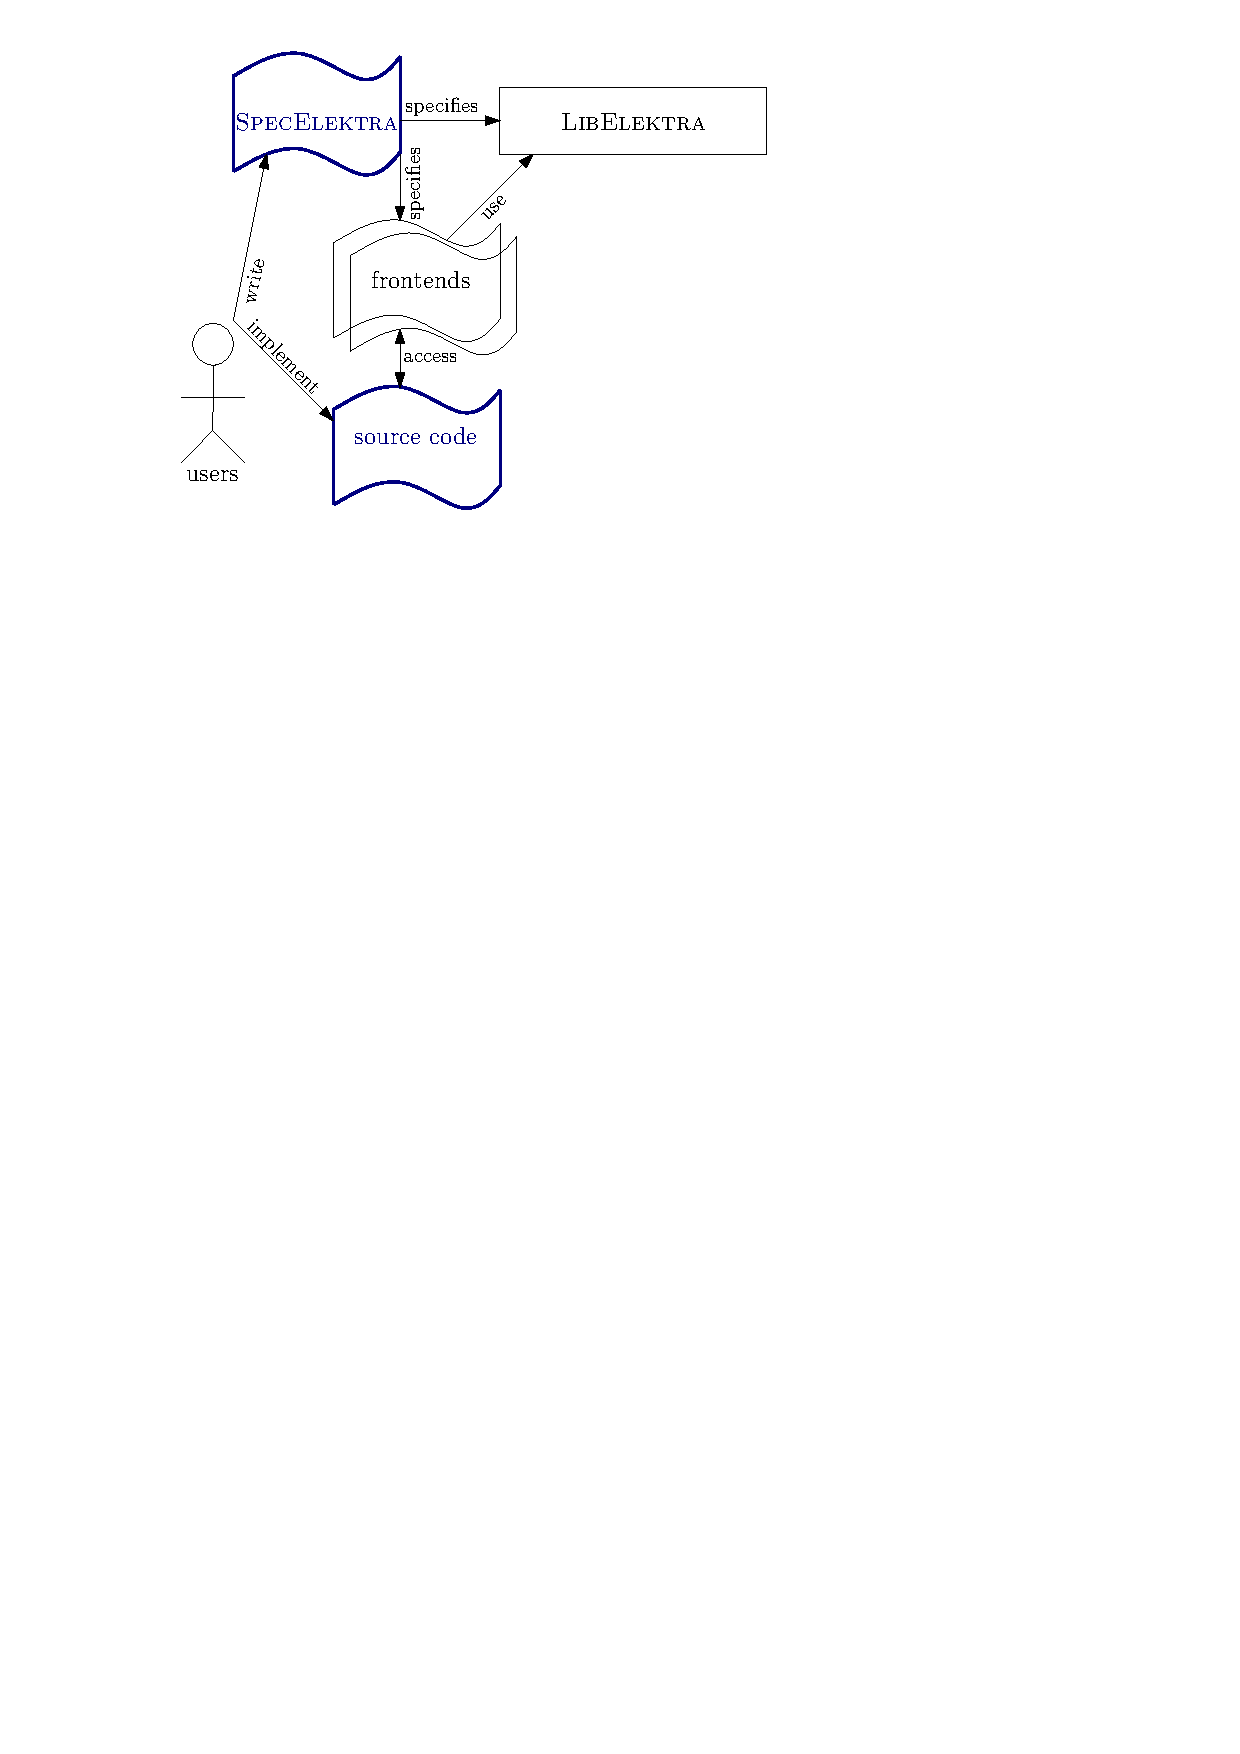
\includegraphics[scale=0.85]{framework}
\caption{The \elektra{} framework from the users' perspective.}
\label{fig:framework}
\end{figure}

\figref{framework} shows what is required from users to facilitate \elektra{}:
The blue parts need to be supplied by users.
\elektra{} does not help in implementing the application logic.
It does, however, disentangle the application from source code specific for configuration access.
Applications use \elektra{Lib} via so-called frontends.
\elektra{Spec} specifies both the frontends and \elektra{Lib}.
We will use a key set to represent \elektra{Spec}.
Furthermore, key sets are used for communication between any parts of \elektra{}, such as between frontends and \elektra{Lib}.

\subsection{\textsc{SpecElektra}}
\label{sec:spec}

%<*definition-spec>
\elektra[Spec]{Spec} is a modular \intro{configuration specification language} for configuration settings.
In \elektra{Spec} we use properties to specify configuration settings and configuration access.
\elektra{Spec} enables us to specify different parts of \elektra{}.
%</definition-spec>

%<*definition-plugins>
\intro[plugin]{Plugins} are filters, sinks, and sources processing a key set.
We aim at \elektra{Spec} to be as modular as possible and make extensive use of plugins:

\begin{enumerate}
\item \elektra{Spec} does not have any built-in feature, all features are (or can be) implemented as plugins.
\item \elektra{} works completely without \elektra{Spec}'s specifications.
\item Configuration specifications are present within the execution environment.
Thus any tool and plugin can introspect and use the specifications.
\end{enumerate}
%</definition-plugins>

\subsubsection{Semantics}

Several tools and plugins read and implement \elektra{Spec}'s specifications.
A meta-specification within \elektra{} defines which property is used by which tool and plugin.
Here we characterize how semantics are defined.
We elaborate on \elektra{Spec}'s semantics in the rest of this chapter.

In this book, we focus on the central properties and tools.
Users can extend \elektra{Spec} by additional properties, but cannot redefine existing ones.
We mainly discuss possibilities \elektra{Spec} offers and only elaborate on non-obvious features.
Because every property has a grammar assigned by $\Psi$, the syntax of property values is formally specified.
Semantics of the properties are described---usually informally---in the meta-specification of \elektra{Spec} and in this book.
Plugins implement the semantics of the properties.
The semantics of the configuration values are described---then again mostly informally---by the properties.
Applications implement the semantics of the configuration values.%
{\parfillskip=.7\textwidth \emergencystretch=.5\textwidth \par}

\begin{example}
\label{ex:property-description}
We give an example of a trivial feature to clarify how the specification is used:

\begin{code}
[slapd/threads/listener]
  description:=Text to be displayed in application.
\end{code}

The specification uses the INI-like syntax introduced in \secref{syntax-spec}.
The syntax of the text to the right of ^:=^ is given by $\Psi(\property{description})$, which is $\Strings$ (any text).
The property puts no constraints on the key \key{slapd/threads/listener}.
If applications present the configuration setting to the user, however, the property \property{description} shall be part of this presentation.
Applications have access to the properties in the same way as the tools and plugins have, therefore they are candidates to give properties meaning.
Furthermore, the application behavior must be in accordance with the semantics described in the description.%
{\parfillskip=0pt plus .7\textwidth \emergencystretch=.5\textwidth \par}
\end{example}

Different from \exref{property-description}, other properties than description usually affect the configuration access behavior.
The semantics of the individual properties are combined by sequential enforcement of each property.
Before introducing more properties, we give an overview how the configuration access works.



\subsection{Key Database}
\label{key-database}
\label{sec:api-key-database}
\label{sec:kdb-semantics}

\elektra{Lib} implements a \intro{key database}.
It provides a unified, system-wide, key-value-based view of the execution environment.
The view contains all previously defined namespaces, including namespace \namespace{spec}, which holds \elektra{Spec}'s specifications.
The key database is the part shared between all applications in a system and consists of several \intro[backend]{backends}.
Each backend maps a key set from a configuration file into the key database with the help of plugins.
The minimal goal of a backend is to parse and serialize configuration files.

To realize several backends \elektra{Lib} splits and merges the key set in such a way that each backend receives only the part of the key set it is responsible for.
At least every namespace is separated in a different backend.
The key database can be seen as a tiny middleware between plugins and applications~\cite{raab2015kps}.

\elektra{Lib}'s main purpose is to present configuration settings and specifications uniformly.
To do so, \elektra{Lib} abstracts over all configuration sources (i.\,e., key set's namespaces) of the execution environment.
All applications and tools with the same context see the same configuration settings and specifications.

\begin{figure}[htp]
\centering
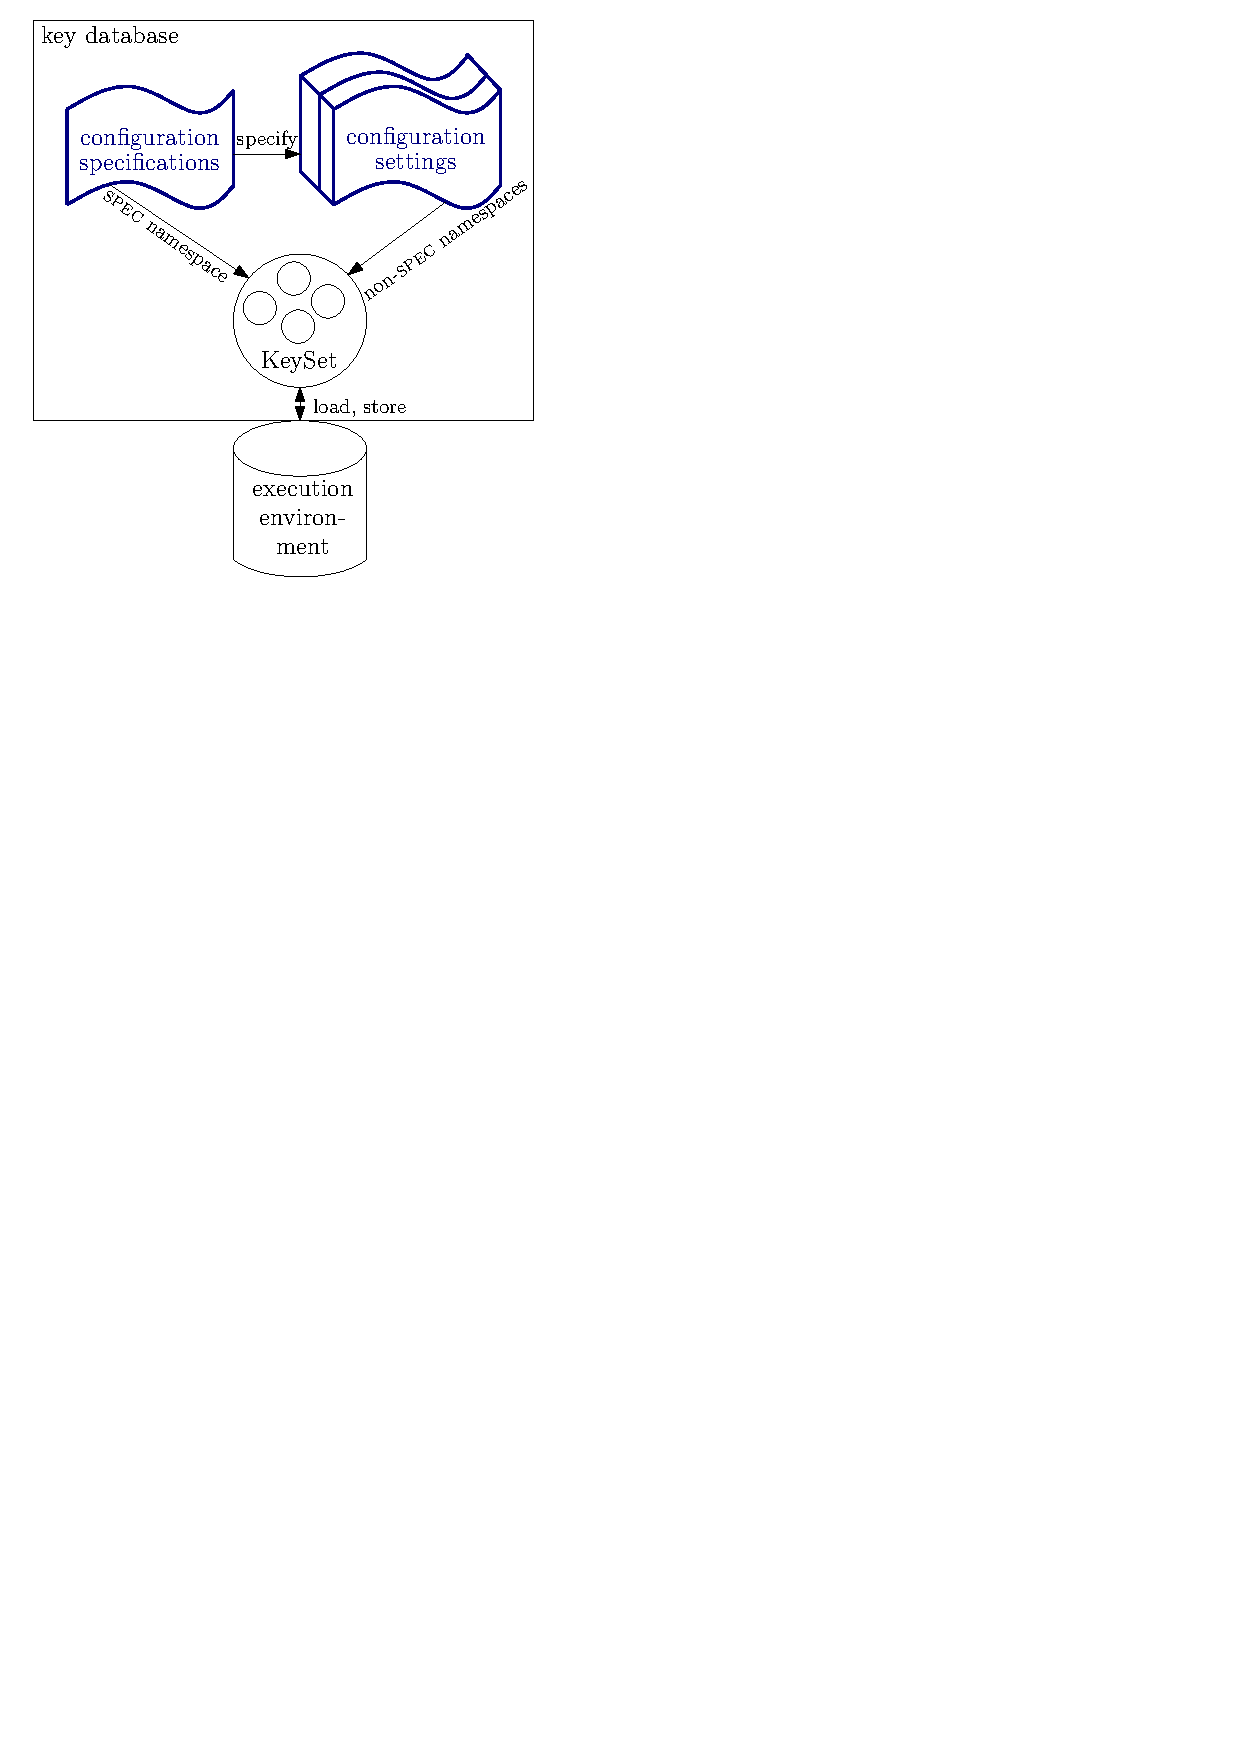
\includegraphics[scale=0.9]{namespaces}
\caption[The namespace in the key database.]{The execution environment stores key sets of all namespaces.
The namespace \namespace{spec} specifies the other namespaces (\namespace{proc}, \namespace{dir}, \namespace{user}, and \namespace{system}).
Arrows indicate data flow of key sets.}
\label{fig:namespaces}
\end{figure}

As shown in Figure~\ref{fig:namespaces} the key database contains configuration specifications in the namespace \namespace{spec}.
All other namespaces are specified by this single specification written in \elektra{Spec}.
Keys with the same key name refer to the same configuration setting.
If key names only differ in the namespace, the key in the namespace \namespace{spec} specifies the other keys.
We enable system administrators to change configuration specifications with the same tooling as used to modify configuration settings.

\begin{example}
Let us assume that the following configuration setting is stored in a configuration file on a system:

\begin{code}[language=CfgElektra]
slapd/threads/listener=4
\end{code}

If this configuration file is read from a system's configuration source (and assuming that the configuration setting is not found in any of the other namespaces) it is part of the namespace \namespace{system}.
As result, we get the key with the name \key{system:/slapd/threads/listener}.
For configuration specifications, we assume the namespace \namespace{spec}:

\begin{code}
[slapd/threads/listener]
  description:=Example from the introduction
\end{code}

The configuration specification has the key name \key{spec:/slapd/threads/listener} and refers to the configuration setting above.
\end{example}

\subsubsection{API}
\label{sec:kdb-api}

\elektra{Lib} provides access to the key database by synchronizing the execution environment and an in-memory key set.
The API to access the key database is minimalist and consists of only four functions.
We abbreviate the key database with ^kdb^ and use ^KDB^\index{KDB@\lstinline{KDB}} as its type in the implementation.

\begin{description}[font=\textintro]
\item[kdb.open():] \index{kdb.open}
The first step is to open a connection to the key database.

\label{sec:bootstrapping}
Because \elektra{Lib} is a library, it needs to \intro{bootstrap} itself during the launch of every application.
First \elektra{Lib} reads from an initial configuration file from a hard-coded path.
Given the content of this initial configuration file, \elektra{Lib} knows about the rest of the execution environment.
The initial configuration file contains information about which plugins must be used~\cite{raab2015kps}.
\item[kdb.get(\texttt{KeySet}):] \index{kdb.get}
The application (initially) fetches and (later) updates its configuration settings as a key set of type ^KeySet^ from the execution environment by one or many calls to ^kdb.get^.
If all relevant configuration files are unmodified since the last invocation, ^kdb.get^ will do nothing.
\item[kdb.set(\texttt{KeySet}):] \index{kdb.set}
When a user finishes editing configuration settings, ^kdb.set^ is in charge of writing all changes back to the key database.
This function atomically persists a whole key set in involved parts of the execution environment.
In the case of an error no action takes place.
\item[kdb.close():] \index{kdb.close}
The last step is to close the connection to the key database.
\end{description}

\elektra{} does not provide extra functions for other features with the consequence that every feature related to the key database must be either part of ^kdb.get^, ^kdb.set^, or ^ksLookup^.
Configuration settings not conforming to the configuration specification are rejected by plugins in ^kdb.set^.
Applications that want to validate configuration settings, must serialize configuration settings to configuration files.
This principle encourages us to serialize configuration settings early.
Applications learn about problems via errors from ^kdb.set^.
As long as only \elektra{} is used, the key database is always coherent with its configuration specifications.

Within ^kdb.set^, plugins notify other applications that the configuration settings have been updated.
Other applications listening to these notifications use ^kdb.get^ to update their configuration settings.
This simple mechanism keeps the in-memory key set in sync with the external representation of a key set in the execution environment.

\begin{example}
A user synchronizes the application's ^KeySet^ with the execution environment using the following source code:
\par
\begin{code}[language=Cpp]
KDB kdb;
KeySet conf;
void onNotification () // triggered by other processes
{
	kdb.get (conf);
} // <continues on the next page>
\end{code}

\begin{code}[language=Cpp,firstnumber=7]
int main ()
{
	kdb.get (conf);
	// work with conf...
	kdb.set (conf);
}
\end{code}

Line~11 notifies other processes and triggers ^onNotification^ there.
\end{example}

\subsection{Mounting}

For better modularity, the key database consists of many backends.
In most cases a backend is responsible to parse and serialize a single configuration file.
Each of the backends---in turn---is built up by several plugins.
Here we introduce how users decide about backends and plugins using \elektra{Spec}.

\intro[mounting]{Mounting} integrates a backend into the key database~\cite{raab2008thesis}.
Hence, \elektra{} allows several backends to deal with configuration files at the same time.
Each backend is responsible for its own subtree of the key database.
To integrate a backend into the key database, we mount it by using the property \property{mountpoint} in the configuration specification.
Its property value is the relative file name to mount.
The key that has the property \property{mountpoint} is the root of this subtree.
Subsequent use of ^kdb.get^ and ^kdb.set^ assume configuration settings below the mountpoint in the respective configuration files.

\begin{example}
\label{ex:mountpoint-specification}
To specify mountpoints, we use the following configuration specification:

\begin{code}
[sw]
  mountpoint:=configfile.txt
[sw/libreoffice]
  mountpoint:=libreoffice.conf
\end{code}

These properties are read by \elektra{}'s tools.
The configuration specification achieves that two new backends are instantiated in the key database.
These backends are used for all namespaces, except the namespace \namespace{spec}.
If an application accesses keys in the key database below \key{/sw/libreoffice}, the application receives the configuration settings of ^libreoffice.conf^.
Otherwise, if an application accesses other keys below \key{/sw}, the application receives the configuration settings of ^configfile.txt^.
For the key \key{/}, \elektra{} always assumes the property \property{mountpoint} to be present, the property does not need to be specified by the system administrator.

\begin{figure}[htp]
\centering
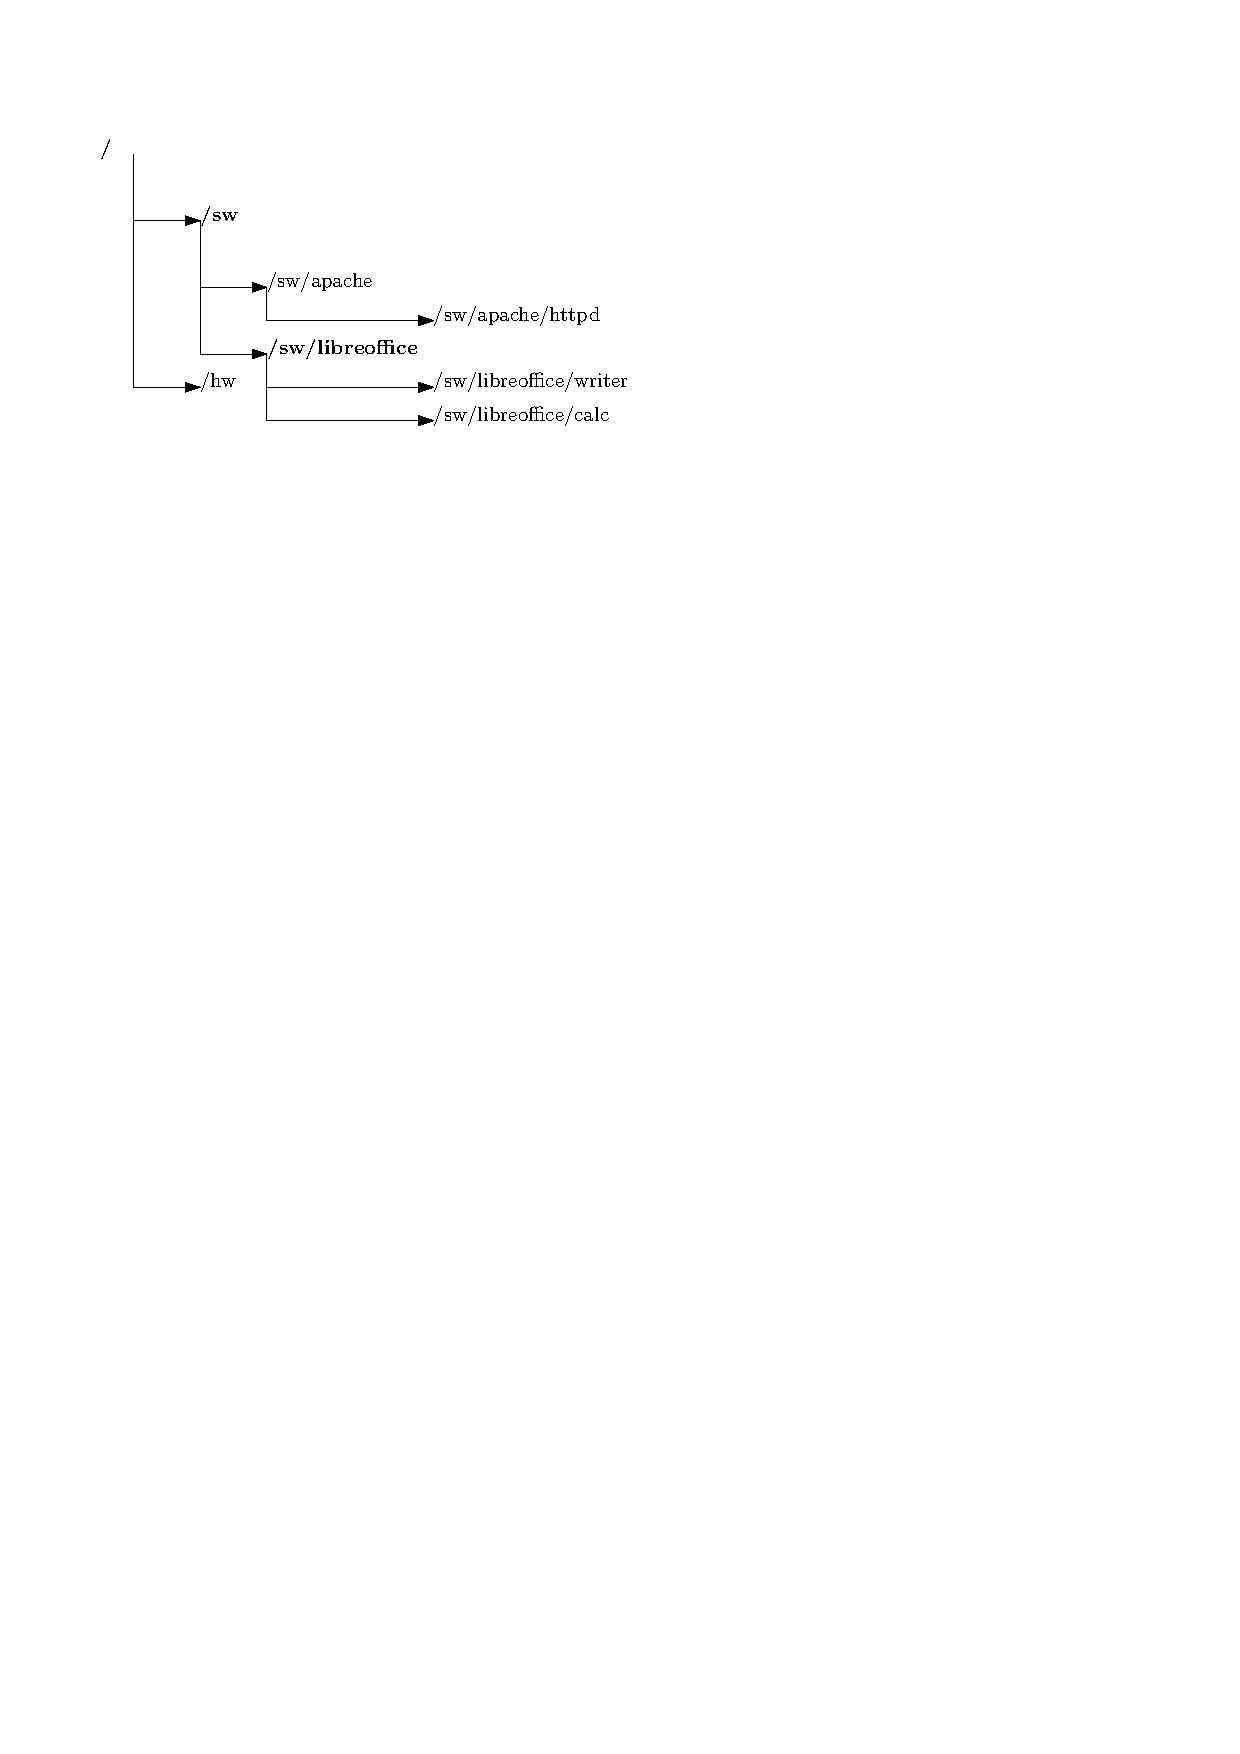
\includegraphics{mounting}
\caption[Mountpoints.]{Mountpoints in \elektra{}. Arrows indicate that keys are below another key.
Bold keys are mountpoints.}
\label{fig:mounting}
\end{figure}

In Figure~\ref{fig:mounting} three subtrees are written in bold: \key{/}, \key{/sw}, and \key{/sw/libreoffice}.\hspace{0.1em}
Backends take care of the configuration settings in their respective subtree.
The subtrees are nested, for example, \key{/sw/libreoffice/writer} belongs to the mountpoint \key{/sw/libreoffice}, while \key{/sw/apache/httpd} belongs to \key{/sw}.
\end{example}

The property \property{mountpoint} abstracts over configuration settings.
Applications do not need to take care about how and where their configuration settings are stored.
It is the task of the backends to implement these details.

Relative key names are relative to their mountpoint.
If we mount the configuration specification to a different root, also the configuration settings get different key names.

\begin{example}
\label{ex:mountpoint-specification-different-mountpoint}
If we mount the configuration specification from \exref{mountpoint-specification} to \key{spec:/test}\footnote{It must be of namespace \namespace{spec} because it is a configuration specification.} then, instead of \key{/sw/libreoffice/writer}, the resulting configuration setting is \key{/test/sw/libreoffice/writer}.
The key \key{/hw}, however, is not concerned about this change.
It still belongs to a \intro{default mountpoint} always present at the namespaces' root.
\end{example}


The property \property{mountpoint} is usually specified by:

\begin{itemize}
\item The system administrator who prefers separated configuration files.
\item Developers that need or want their applications to continue using their previous configuration file.
Setting the property is done during the installation process.
\end{itemize}


Despite the different namespaces in which a configuration setting can be, users need access to properties of any key they currently work with.
Here we describe a metadata abstraction.
At run-time the properties specified in the namespace \namespace{spec} are copied\footnote{Copying metadata is efficient by referring to already existing metakeys.} as metadata into the configuration setting of all namespaces.
Applications and users facilitate this metadata to learn about configuration specification.

\begin{figure}[htp]
\centering
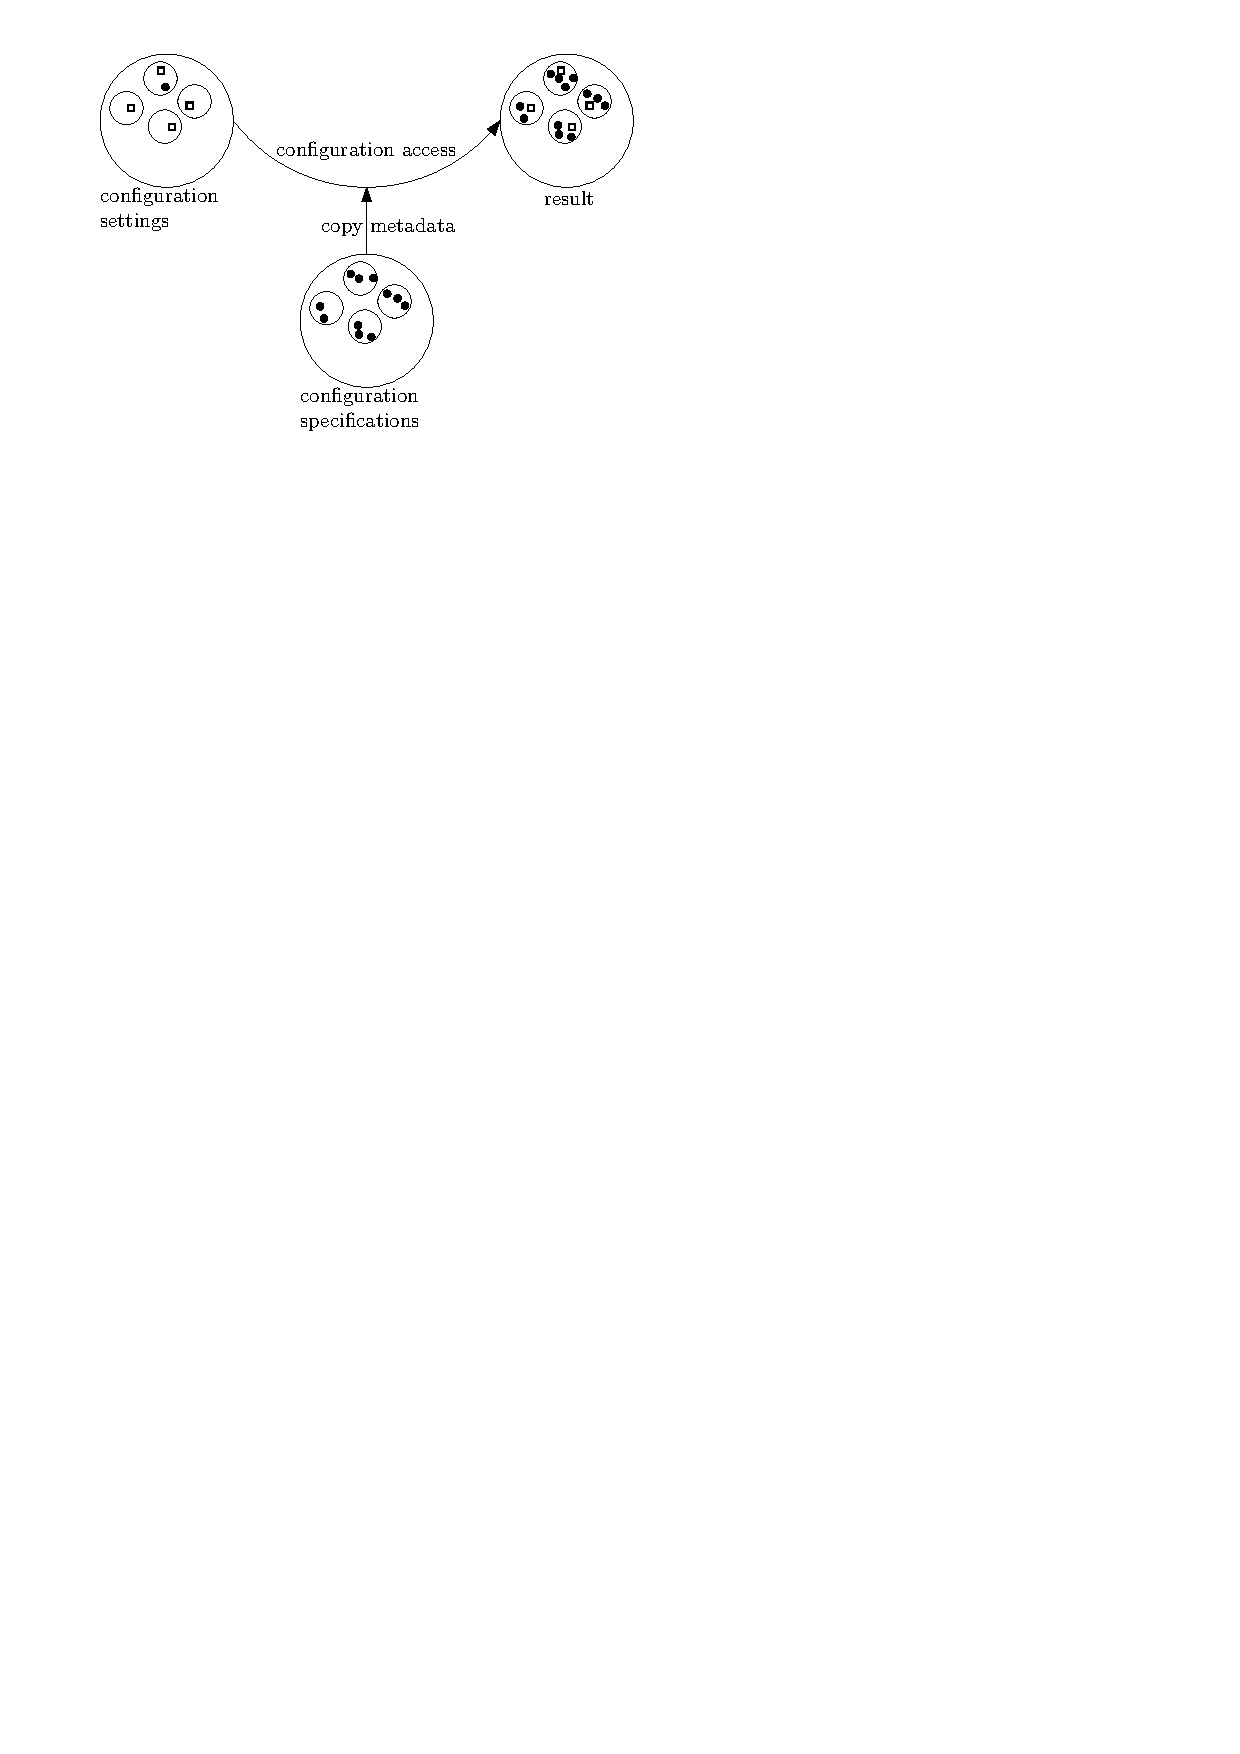
\includegraphics{metadata}
\caption[Abstraction of Metadata.]{Abstraction of Metadata. The large circles are key sets, the smaller ones keys.
Configuration values are boxes and metadata are black dots.}
\label{fig:metadata}
\end{figure}

As we see in \figref{metadata} in the result the abstraction makes it irrelevant whether metadata:
\begin{itemize}
\item has been copied from the properties (i.\,e., metadata in the configuration specifications), or
\item is directly part of configuration settings.
\end{itemize}


\begin{example}
Let us assume we have the configuration specification from \exref{property-description}:

\begin{code}
[slapd/threads/listener]
  description:=Text to be displayed in application.
\end{code}

When an application accesses the key with the key name ^/slapd/threads/listener^ in any namespace, the property \property{description} is part of its metadata.
\end{example}

In the rest of this book, we assume for the configuration settings and specifications given in listings that
\begin{itemize}
\item configuration specifications are mounted at the root of the namespace \namespace{spec},
\item configuration settings are mounted at the root of any other namespace, and
\item properties are available as metadata in every key related to a configuration setting.
\end{itemize}





\subsection{Context Specifications}
\label{sec:context-specification}

\intro[context specification]{Context specifications} are properties of \elektra{Spec}, which make configuration settings more context aware.
They are implemented in frontends (generated by \elektra{Gen}) and in backends (implemented in \elektra{Lib}).

Namespaces and cascading lookup provide a form of context awareness.
For example, they allow the configuration settings to be aware of the current user (namespace \namespace{user}).
Their context awareness is restricted by fixed rules and the fixed number of namespaces.
Here we generalize the concept.

For system administrators a central mechanism to work with \elektra{} is changing properties, i.\,e., modifying metadata in the namespace \namespace{spec}.
We show how system administrators---by writing context specifications in \elektra{Spec}---share configuration settings between applications.
Sharing configuration settings is a kind of context awareness:
We enable applications to be aware of configuration settings of other applications.
We only assume that applications, receiving configuration settings, use the key database.%
{\parfillskip=0.8\textwidth \emergencystretch=.5\textwidth \par}

The properties below achieve this goal.
They are implemented by ^ksLookup^ and are thus part of the key database (implemented in \elektra{Lib}).
The priority of prop\-erties is always fixed and cannot be changed by changing the order of properties in the configuration specifications.
Thus we sometimes need properties with identical semantics but different priority.
Some properties permit us to use array indexes that enable users to choose order within the functionality of that property.
Lower array indexes have higher priority.
We indicate support for array indexes by adding a \textbf{/\#} suffix.
In the order of priority (higher priority first), the properties for context awareness are~\cite{raab2015kps}:

\begin{description}
\label{sec:lookup-properties-priorities}
\item[context] specifies configuration settings to be preferred to the key itself to better fit the context.
With this property we aim at having semantics of contextual values for configuration settings.
We discuss its syntax and semantics in \secref{approach-contextual-values}.
It is implemented using the extension interface ^lookupByExtension^ of ^ksLookup^ as explained in \secref{approach-context-aware-lookup}.
\item[override/\#] specifies configuration settings to be unconditionally preferred to the key itself.
This property enables users to create links between configuration settings.
The grammar assigned to this property value by $\Psi(\property{override})$ is the grammar of key names, as shown in \secref{key-name}.
\item[namespace/\#] defines alternative namespace priorities using array indexes for the specified key.
The grammar of the property value is $\NameSpaces$.
\item[fallback/\#] specifies configuration settings to be used if the key itself is only present in the namespace \namespace{spec}, and not in any other specified namespace.
As in property \property{override}, we create a link between keys and use the grammar of key names.
\item[default] represents a value to be used if no key was found (including consideration of the properties above).
The property value is a string $\in \Strings$, i.\,e., $\Psi(\property{default}) \mapsto \Strings$, and is used as \intro[default value]{default value}.
Because property values cannot be $\NullValue$, default values cannot be $\NullValue$.
\end{description}

\begin{example}
If system administrators want a configuration setting that:
\begin{itemize}
\item prefers the key \key{/sw/pools/threads/listener} if available,
\item only considers the namespace \namespace{system} (and not \namespace{proc}, \namespace{dir}, and \namespace{user}), and
\item has the configuration value ^2^ if the configuration setting is not found otherwise.
\end{itemize}
Then system administrators specify:
\par
\begin{code}[morekeywords={namespace,override}]
[slapd/threads/listener]
  default:=2
  namespace/#0:=system
  override/#0:=/sw/pools/threads/listener
\end{code}
\par
The order of the properties in the configuration specification does not matter.
The property \property{override} has a higher priority than properties \property{namespace} and \property{default} (as given in the list of properties before the example).
We increase context awareness using the property \property{override}.
Without this specification, ^slapd^ would not be aware of the configuration setting \key{/sw/pools/threads/listener}.
We decrease the context awareness of the namespaces:
We do not consider the namespaces \namespace{proc}, \namespace{dir}, and \namespace{user} for the key \key{/slapd/threads/listener}.
Because the key \key{/sw/pools/threads/listener} has no configuration specification, we will consider all namespaces there.
\end{example}

\subsection{Frontend}

We already introduced features that are part of \elektra{Lib} (the backends).
Features in the frontend are part of the application and thus not part of the key database.
When adding features in the frontend we have to be careful:
Applications do not always use the same frontends.
We could easily break the desired globally unified view that the key database promises.
Reasons to put functionality in the frontend nevertheless are:

\begin{itemize}
\item Performance.
\item Ensure presence of configuration settings and specifications even when retrieving configuration settings and specifications from the key database fails.
\item Ensure type safety and improving the usability for developers, for example, directly returning correct types.
\item Supporting features where configuration settings need to differ in different parts of an application.
\end{itemize}

Here we focus on the user's view of type-safe access code for contextual values.
We prefer type-safe access code as frontends and avoid direct access to the low-level key-value operations (^ksLookup^) of \elektra{Lib}.
We call applications that use \elektra{}'s key database via one of its frontends \intro[elektrify]{elektrified}.
\figref{architecture} shows the architecture with code generation used in elektrified applications.
When using \elektra{Lib} in this architecture, users need to:
\begin{itemize}
\item Write a specification in \elektra{Spec} that defines the configuration access of their application.
\item Provide an elektrified source code for their applications that directly makes use of the generated, type-safe frontends.
\end{itemize}
This architecture is the preferred way for newly written applications.
In \secref{unmodified-floss}, we will present an alternative architecture for applications without changing their frontend.


\begin{figure}[htp]
\centering
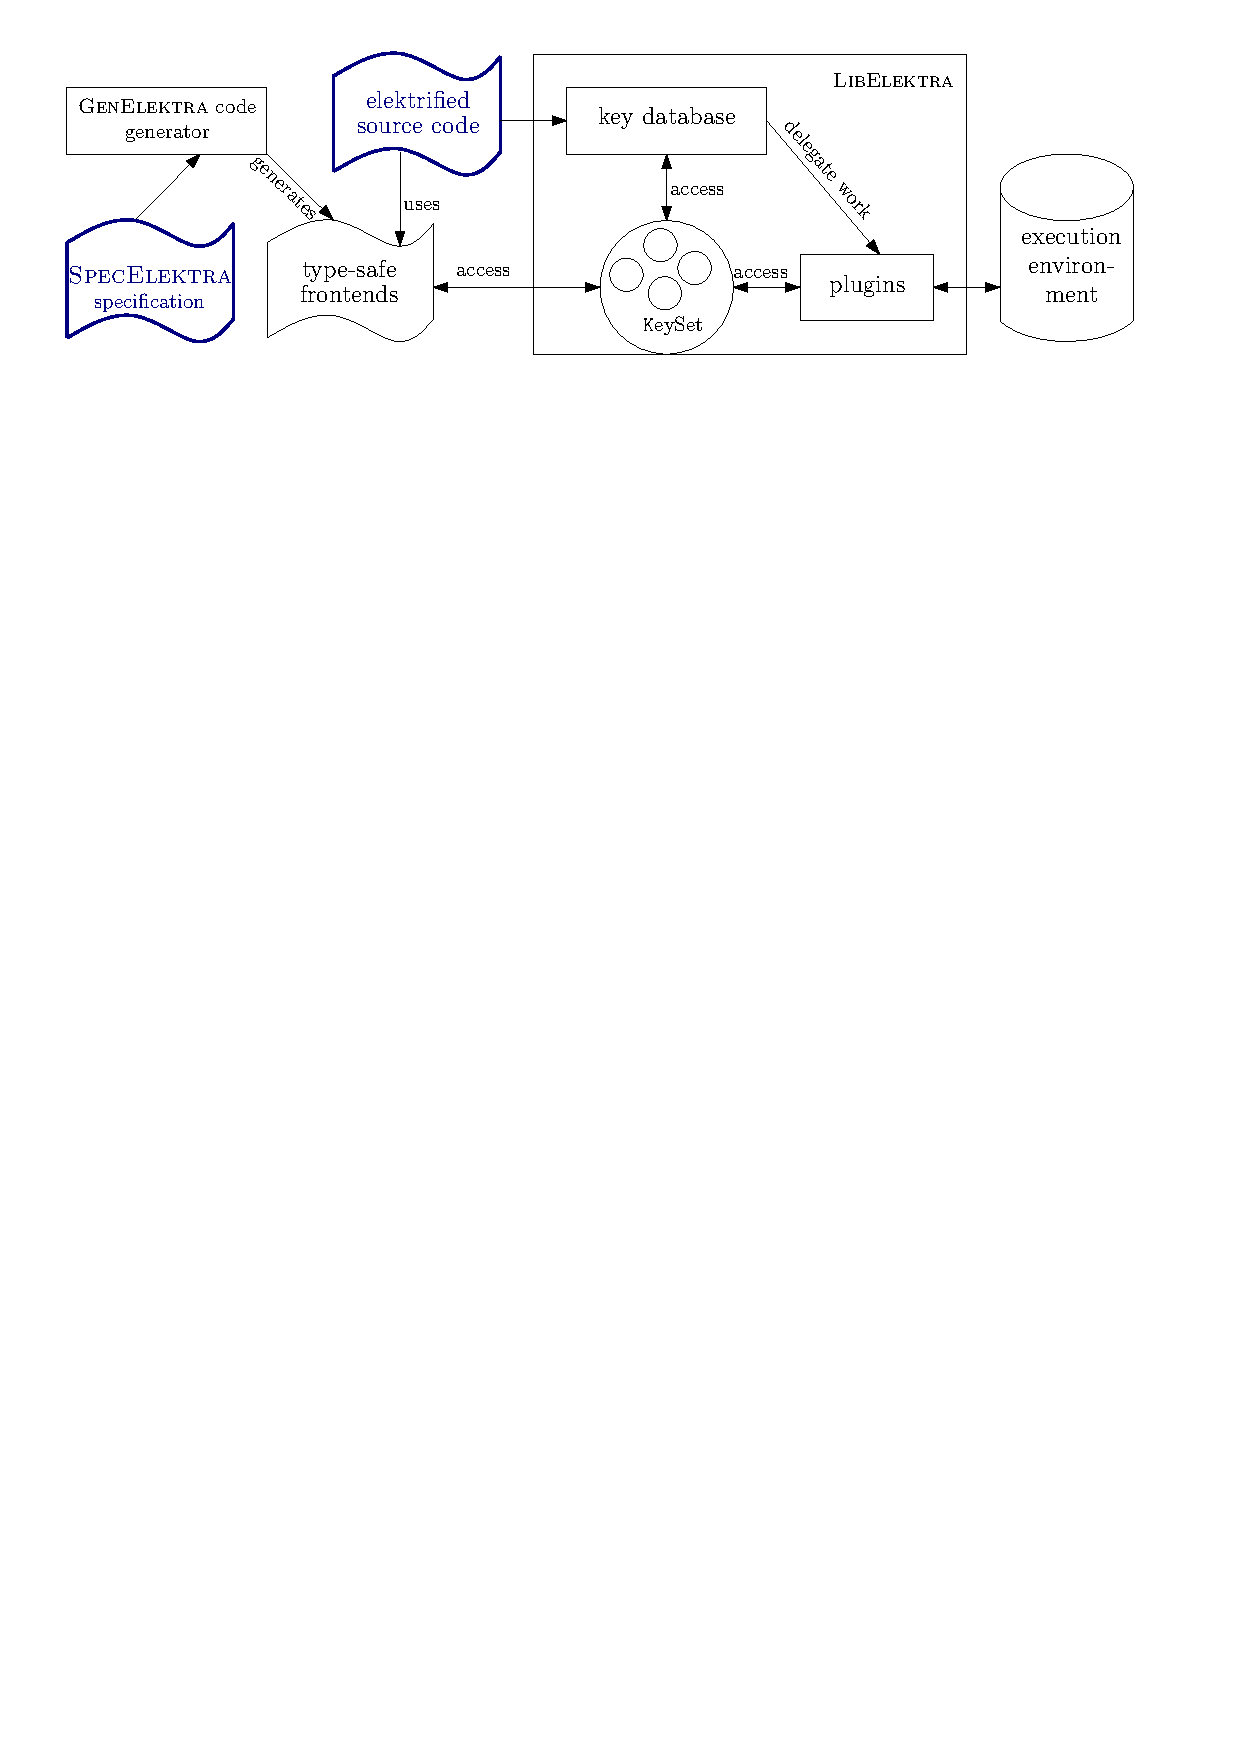
\includegraphics[width=\textwidth]{architecture}
\caption[Architecture of \elektra{}.]{Architecture of \elektra{} with code generation.
Bold, blue boxes need to be provided by users of \elektra{}.}
\label{fig:architecture}
\end{figure}

\subsubsection{Code Generation}
\label{sec:approach-code-generation}

The code generator \elektra[Gen]{Gen} reads \elektra{Spec} specifications and emits high-level APIs to be used in applications.
\elektra{Gen} facilitates the key names to generate unique API names.
We use nested objects (accessed by ^.^ via a root object ^env^) according to the hierarchy levels of the key name.
These objects are used like variables.
\elektra{Gen} employs the following properties from \elektra{Spec}:

\label{sec:property-opt}
\begin{description}
\item[type] represents the type to be used in the emitted source code.
The emitted variables implicitly cast to the type given here.
For property \property{type}, we use the common object request broker architecture (CORBA) interface description language (IDL) data types, which already have well-defined mappings for many programming~languages.
\item[opt] is used for short command-line options to be copied to the namespace \namespace{proc}.
Here we can choose between implementations in the frontend and backend with the trade-off performance versus flexibility for system administrators.
\begin{example}
With the property ^opt:=p^, the configuration setting with this property can be changed by adding the command-line option ^-p^.
\end{example}
\item[opt/long] is used for long command-line options, which differ from short command-line options by supporting strings and not only characters.
\item[readonly] yields compilation errors when developers assign a value to a contextual value within the program.
\item[default] enables us to start the application even if the backend does not work.
\elektra{Gen} uses it to hard-code default values into the application.
If the backend is available, the property \property{default} is interpreted by the backend.
Without the property \property{default}, the configuration value can be missing (^ksLookup^ can return~$\NullKey$).
In the high-level APIs the user would get a run-time error when trying to access such a configuration value.
Thus if the property \property{default} is not available, \elektra{Gen} will not generate a contextual class for the given configuration specification to protect the user from run-time errors.
\end{description}


\begin{example}
The specification ^[foo/bar]^ alone (without properties) does not generate any code because property \property{default} is not given.
Calling ^ksLookup^ on such a configuration setting is not safe and can return $\NullKey$ (indicating the not-found key).
\end{example}


\begin{example}
\label{ex:code-generation}
With the specification:
\par
\begin{code}
[foo/bar]
  default:=Hello
  type:=string
  opt:=b
  readonly:=1
\end{code}
\par
\elektra{Gen} gives the user read-only access to the object ^env.foo.bar^:
\par
\begin{code}[language=Cpp]
std::cout << env.foo.bar;
env.foo.bar = "Other world"; // compilation error
\end{code}
\par
Line~1 prints the configuration value of ^/foo/bar^ or ^"Hello"^ (without quotes) by default.
When invoking the application with ^application -b "This world"^, the application would print ^"This world"^ (without quotes).
Line~2 leads to a compilation error because of the property \property{readonly}.
\end{example}




\subsection{Contextual Values}
\label{sec:approach-contextual-values}

The most expressive part of the \intro{context-aware lookup} algorithm is the \empha{layer-based lookup}.
It enables configuration access points to have semantics of \empha[contextual value]{contextual values}.
\intro[context-aware configuration]{Context-aware configurations} are configuration settings in which context-aware look\-ups are used.
We provide two types of context-aware configurations, implemented in frontend and backend, respectively.
Both types share the following syntax:

\begin{definition}
\intro[layer value]{Layer values} are relative key names $\in \RelativeKeyNames$.
\intro[layer name]{Layer names} are non-empty, clean strings $\in \NonEmptyCleanStrings$ embedded in a context specification as given in the following grammar (we use \synt{basename} and \synt{hierarchy level} from \defref{basename} and $\NameSpaces$ from \defref{key-name}):

{
\label{def:layer-syntax}
\setlength{\grammarindent}{14em} % increase separation between LHS/RHS
\begin{grammar}
<contextual key name> ::= [ $\NameSpaces$ \lq^:^' ] \lq^/^' \{ <contextual hierarchy level> \lq^/^' \} \\ <basename>

<contextual hierarchy level> ::= <context placeholder>
                          | <hierarchy level>

<context placeholder>     ::= \lq^%^' <layer name> \lq^%^'
\end{grammar}
}
\end{definition}

Every hierarchy level is a contextual hierarchy level and every key name is a contextual key name, thus Definition~\ref{def:layer-syntax} generalizes \defref{key-name}.

Both forms of contextual values (frontend and backend) share the following semantics:
\begin{definition}
\label{def:context-evaluate}
\intro[layer]{Layer} is a mapping from layer names to layer values and represents the current context.
The function \texttt{context.evaluate} replaces all context placeholders with layer values given by the layers.
If no layer name is found, or the layer value is empty, the layer value ^%^ will be used.
We call a layer \intro[active layer]{active} if the layer does not have the layer value ^%^.
\end{definition}

\begin{example}
\label{ex:contextual-key-name}
Given the contextual key name ^/foo/%bar%/hey^, depending on the layer value of the layer name ^bar^, the following incomplete list of key names are valid contextual interpretations:

\begin{code}[language=CfgElektra]
foo/%/hey=     ; no such layer, or no layer value
foo/bar/hey=   ; layer value bar
foo/foo/hey=   ; layer value foo
foo/some/more/hierarchy/hey=
\end{code}

The layer value in line~4 is \str{some/more/hierarchy}.
\end{example}



\subsubsection{Backend}
\label{sec:approach-context-property}

In the first type of contextual values the meta-function $\Psi$ assigns the grammar of contextual key names as given in \defref{layer-syntax} to the property value of the property \property{context}.
When looking up such a key, \elektra{Lib} substitutes the context placeholder and tries to search the resulting key name.
Similar to the property \property{override}, the key is preferred to the configuration value of the original key.

For the property \property{context}, layers are specified within the key database.
The layer names are wildcards to discriminate between different possible keys.

\begin{example}
We define a context-aware link using the property \property{context}:

\begin{code}[morekeywords={override}]
[foo]
  context:=/foo/%bar%/hey
  override/#0:=/foo/hey
\end{code}

When looking up ^foo^, depending on the layers, key names in the form as given in \exref{contextual-key-name} are looked up.
On failure, the lookup continues with the property \property{override} because of the priorities as specified in the list of properties in \secref{lookup-properties-priorities}.
\end{example}

\subsubsection{Frontend}
\label{sec:approach-users-view-frontend}

In the second type of contextual values we do not use properties.
Instead we directly use contextual key names as key names in the configuration specification.
In the configuration settings' syntax, we denote the contextual key names without their namespace \namespace{spec}.
It is the task of the frontend to call \texttt{context.eval\-uate} so that context placeholders are resolved before calling ^ksLookup^.
\elektra{Lib} provides a predefined class ^Context^, which is the interface for users to dynamically activate and deactivate layers~\cite{raab2014program}:

\begin{code}[language=Cpp]
class Context : public Subject
{       // for the frontend:
	string evaluate(string const & spec) const;
public: // for the user:
	template <typename Layer> void activate(...);
	template <typename Layer> void deactivate(...);
	template <typename Layer> Context & with(...);
	template <typename Layer> Context & without(...);
	...
};
\end{code}

The purpose of the class ^Context^ is to govern the layers in a data structure (i.\,e., not in the key database).
To change the context, the class ^Context^ provides four methods for the user:

\begin{description}
\item[activate:] \index{layer!activation}  Activates a layer without scope.
\item[deactivate:] \index{layer!deactivation} Deactivates a layer without scope.
\item[with:] Activates a layer in a dynamic scope.
\item[without:] Deactivates a layer in a dynamic scope.
\end{description}

While the methods ^activate^ and ^deactivate^ affect the rest of the execution (until another context change is done), the methods ^with^ and ^without^ are bound to their dynamic scope.


In \chapref{frontend} we describe the semantics of these methods and different ways how the user specifies the ^typename Layer^ required in the interface of ^Context^.

\intro[contextual classes]{Contextual classes} emitted by \elektra{Gen} implement contextual values and can directly be used by the developer.
In generated classes, we use the naming conventions for nested objects as described in \secref{approach-code-generation} but with the context placeholders removed.
Contextual classes implement contextual values.

\begin{example}
If we change \exref{code-generation} to have the contextual key name ^[foo/^\allowbreak^%language%/bar]^, we get a contextual value ^env.foo.bar^.
Then the output differs depending on the layer value of ^language^.
Assume the configuration settings:
\par
\begin{code}[language=CfgElektra]
foo/english/bar=Hello
foo/german/bar=Hallo
\end{code}
\par
With the layers $\{\text{language} \mapsto \text{german}\}$, the application will output ^"Hallo"^ (without quotes).
\end{example}

\subsubsection{Frontends versus Backends}

Here we discuss differences between contextual interpretations in the backend and in the frontend.
Contextual key names---used as key names in configuration specifications---are only useful if used along with frontends.
Such key names cannot be resolved within backends:
They are not valid key names and thus cannot be looked up.
The advantage of frontends' contextual values is that layers can be restricted within dynamic scopes.%
{\parfillskip=0pt \emergencystretch=.5\textwidth \par}


For the lookup within the backend, the frontend is completely unaware that a context-aware lookup takes place.
Thus the property \property{context} provides a stronger abstraction.























\section{Backend}
\label{sec:kdb}

\index{backend|boldindex}

In this section we reflect upon the system's view of \elektra{}, with a focus on the key database.
We go into the details of the lookup algorithm with its two main helper functions ^lookupBySpec^ and ^lookupByExtension^ implementing the already explained properties.
In previous work we discussed an earlier version of the lookup algorithm~\cite{raab2015kps}.
After explaining the details of the metadata abstraction, we discuss how plugins are assembled to backends.

\elektra{} already has many predefined plugins as shown in the figure on page~\pageref{fig:plugins}.
Users add further plugins to extend \elektra{}'s functionality.
The plugins we use in the examples are implemented.
For brevity, we sometimes shorten information about plugins in the examples.
For the full contracts please refer to the source code repository at \url{https://git.libelektra.org}.

\subsection{Layer-based Lookup Algorithm}

The \intro{layer-based lookup} facilitates layers using ^context.evaluate^.
Layer-based lookup is a special form of the context-aware lookup.

We use $l \in \Keys$, $z \in \Keys_\NullKey$, $c \in \KeySets$, $p \in$ \synt{property name}, and $i \in$ \synt{array index}.
Let us start with defining small helper functions:
\begin{description}[font=\ttfamily]
\item[lookupProperty] $(l, p) \to z$ returns a new key $z$, where $z.k = l.\mu(p)$, which is the property value from the property name $p$.
The function returns $\NullKey$ if the property is not present in $l$.
\item[lookupByKey] $(c, l) \to z$, where $z.k = l.k$.
The function returns $\NullKey$ if the key name is not present in $c$.
\item[length] $(l, p) \to i$ returns the last array index of the property name $p$ in $l$.
The property name $p$ needs to contain a ^#^, which indicates an array index.
If no array index is found, a special value is returned that avoids iterations of a ^for^ loop.
The loop ^for (i: "#0" .. length (l, p))^ iterates over all array indexes present in $l.\mu$.%
{\parfillskip=0pt plus .8\textwidth \emergencystretch=.5\textwidth \par}
\end{description}

The layer-based lookup is implemented as extension point ^lookupByExtension^ introduced in \secref{approach-lookup}:

\label{sec:approach-context-aware-lookup}
\begin{code}[language=Cpp,morekeywords={is,of},escapeinside={(*@}{@*)}]
Key lookupByExtension (KeySet c, Key l, Key specKey)
{
	if ((specKey == (*@$\NullKey$@*)) || !(l is of namespace (*@$\EmptyNameSpace$@*))) return (*@$\NullKey$@*);
	Key k = lookupProperty (specKey, "context");
	if (k != (*@$\NullKey$@*))
	{
		k.k = context.evaluate (k.k);// evaluate property value
		k   = lookup (c, k);   // recursion to lookup algorithm
	}
	return k;
}
\end{code}

The key ^specKey^ is the key ^spec^ $\concatkey$ ^l^.
In line~3 we handle invocations of the extension interface we do not need to implement for a layer-based lookup.
In line~4 we check for the presence of property \property{context}.
If the property is available, in line~7, the function \texttt{context.evaluate} replaces the context placeholders.
Then we recursively descend with the new key name (line 8).
In line 10 we return the found key or $\NullKey$, and let the caller continue with the cascading lookup~\cite{raab2016unanticipated}.

\subsection{Specification Lookup Algorithm}

The algorithm ^lookupBySpec^ implements the search logic for the properties in the cascading lookup.
Let us add further helper functions.
The first helper implements the properties \property{override} and \property{fallback} (as specified with \texttt{type}):

\begin{code}[language=Cpp,morekeywords={is,of},escapeinside={(*@}{@*)}]
Key lookupByLink (KeySet c, Key specKey, string type)
{	// type is either "override" or "fallback"
	for (i: "#0" .. length (specKey, type (*@$\concat$@*) "/#"))
	{
		Key k = lookupProperty (specKey, type (*@$\concat$@*) "/" (*@$\concat$@*) i);
		k = lookup (c, k); // recursion
		if (k != (*@$\NullKey$@*)) return k;
	}
	return (*@$\NullKey$@*); // not found
}
\end{code}

In the loop starting on line~3, we consider all array indexes of the links.
If we find a link, we recursively look it up (line~6).
If the lookup was successful, we return the found key (line~7).

We already discussed the exhaustive search of all namespaces in \secref{approach-lookup}:

\begin{code}[language=Cpp,morekeywords={is,of},escapeinside={(*@}{@*)}]
Key lookupNamespaces (KeySet c, Key l)
{
	Key k = lookupByKey (c, "proc" (*@$\concatkey$@*) l);
	if (k == (*@$\NullKey$@*)) k = lookupByKey (c, "dir" (*@$\concatkey$@*)  l);
	if (k == (*@$\NullKey$@*)) k = lookupByKey (c, "user" (*@$\concatkey$@*)  l);
	if (k == (*@$\NullKey$@*)) k = lookupByKey (c, "system" (*@$\concatkey$@*)  l);
	return k;
}
\end{code}

Evaluating the property \property{namespace/#} is similar to the algorithm ^lookupByLink^.
The behavior on absence of the property is different:
Instead of doing nothing we exhaustively search all namespaces using the function ^lookupNamespaces^ specified directly above:

\begin{code}[language=Cpp,morekeywords={is,of},escapeinside={(*@}{@*)}]
Key lookupByNamespace (KeySet c, Key l, Key specKey)
{
	if (lookupProperty (specKey, "namespace/#0") != (*@$\NullKey$@*))
	{
		for (i: "#0" .. length (specKey, "namespace/#"))
		{
			k = lookupProperty (specKey, "namespace/" (*@$\concat$@*) i);
			k = lookupByKey (c, k.k (*@$\concatkey$@*) l);
			if (k != (*@$\NullKey$@*)) return k;
		}
	}
	else // if no property namespace exists
	{
		k = lookupNamespaces (c, l);
		if (k != (*@$\NullKey$@*)) return k;
	}
	return (*@$\NullKey$@*); // not found
}
\end{code}

To implement the properties defined in \secref{lookup-properties-priorities} (except properties \property{context} and \property{default}) we only need to call the functions in order of priority:

\label{sec:lookup-by-spec}
\begin{code}[language=Cpp,escapeinside={(*@}{@*)}]
Key lookupBySpec (KeySet c, Key l, Key specKey)
{
	Key k = lookupByLink (c, specKey, "override");
	if (k == (*@$\NullKey$@*)) k = lookupByNamespace (c, l, specKey);
	if (k == (*@$\NullKey$@*)) k = lookupByLink (c, specKey, "fallback");
	return k;
}
\end{code}

The method ^lookupBySpec^ is only relevant within a \empha{cascading lookup} and if a ^specKey^ is present.


\subsection{Lookup Algorithm}

\begin{code}[language=Cpp,morekeywords={is,of},escapeinside={(*@}{@*)}]
Key lookup (KeySet c, Key l, Key specKey)
{
	Key k = lookupByExtension (c, l, specKey);
	if (k == (*@$\NullKey$@*) && !(l is of namespace (*@$\EmptyNameSpace$@*)))
	{
		return lookupByKey (c, l); // non-cascading lookup
	}
	if (k == (*@$\NullKey$@*) && specKey != (*@$\NullKey$@*))
	{
		k = lookupBySpec (c, l, specKey); // cascading lookup
	}
	if (k == (*@$\NullKey$@*)) k = lookupNamespaces (c, l);
	return k;
}
\end{code}

We see (because of the branch starting in line~4) that the function ^lookup^ supports the two already-discussed forms of lookups: cascading and non-cascading lookups.
Because the function ^lookup^ calls ^lookupByExtension^ and ^lookupBySpec^, all properties are handled recursively.
As final helper function, we define ^lookupPropertyAsValue^ $(l, p) \to z$ that works similar to ^lookupProperty^ but with the property value used as value and not as key name.
The record $z$ has the following fields:
\begin{description}[noitemsep,topsep=0pt,parsep=0pt,itemsep=0pt]
\item[$k$] is the name of $l$ (i.\,e., $l.k$), and
\item[$v$] is the property value of the property name $p$ as found by $l.\mu(p)$.
\end{description}

Now we have all functions ready to finally define the algorithm ^ksLookup^:


\label{sec:lookup}
\begin{code}[language=Cpp,morekeywords={is,of},escapeinside={(*@}{@*)}]
Key ksLookup (KeySet c, Key l)
{
	Key specKey = lookupByKey (c, "spec" (*@$\concatkey$@*) l);
	Key k = lookup (c, l, specKey);
	// <continues on the next page>
\end{code}

\begin{code}[language=Cpp,morekeywords={is,of},escapeinside={(*@}{@*)},firstnumber=6]
	if ((k == (*@$\NullKey$@*)) && (l is of namespace (*@$\EmptyNameSpace$@*)) && (specKey != (*@$\NullKey$@*)))
	{
		k = lookupPropertyAsValue (specKey, "default");
	}
	return k;
}
\end{code}

The last step (line~6) of the lookup algorithm is to use the default value if everything else failed:
The property \property{default} is exclusively considered on top-level of the recursion.%
{\parfillskip=0pt \emergencystretch=.5\textwidth \par}










\subsection{Abstraction of Metadata}

Within \elektra{} both configuration settings and specifications are represented by a key set.
In \secref{syntax} we introduced separated syntaxes for configuration specifications (with ^property:=value^) and configuration settings (with \lstinline[language=CfgElektra]^key=value^).
Here we demonstrate why this separation of configuration settings and specifications is not visible to plugins and applications in \elektra{}.
We present an abstraction in which applications and plugins cannot distinguish between syntaxes.
In particular, the abstraction obscures if metadata is separated or embedded.

\subsubsection{Embedded Metadata}

Many configuration file formats have metadata embedded.
Often metadata is needed to properly reconstruct the configuration file~\cite{raab2010thesis}.
\elektra{} stores metadata within $\mu$ of the keys.%
{\parfillskip=0pt plus .8\textwidth \emergencystretch=.5\textwidth \par}

\begin{example}
\label{ex:json}
Let us consider the following JSON file~\cite{raab2015kps}:

\begin{code}[language=CfgElektra]
{ "key": true }
\end{code}

In JSON a non-quoted ^true^ is a boolean, which is different from the string ^"true"^.
\elektra{}'s JSON plugin transforms this file into a key set, remembering JSON's type in the metadata ^type^.
As already mentioned, the values ^0^ and ^1^ represent a boolean in \elektra{}.
If we serialize this key set to XML syntax we get:

\begin{code}[language=XML]
<?xml version="1.0" encoding="UTF-8" standalone="no" ?>
<key type="boolean">1</key>
\end{code}
\phantom{}
\end{example}

\subsubsection{Abstraction over Embedded and Separated Metadata}

In this book we keep configuration settings and specifications separated from each other.
From the user's point of view the distinction is useful to easily get a grasp of the involved meta-level.
From an application's point of view, however, it is useful if the metadata comes along with the configuration setting, for example, when using a context-aware lookup we do not know which key name we get.
We do not burden applications and plugins to distinguish between the embedded or separated form.

To abstract over these two competing ways, we utilize the following concept:
We copy all properties to the key's metadata in all other namespaces.
\elektra{} implements this concept in the plugin \plugin{spec}.
The key name of the ^spec^ key is used as pattern to be matched against the other keys.
Properties are copied to matching keys.

\begin{example}
Suppose we have the following configuration specification:

\begin{code}
[slapd/threads/listener]
  check/range:=1,2,4,8,16
\end{code}

And we have the following configuration setting mounted to namespace \namespace{system}:

\begin{code}[language=CfgElektra]
slapd/threads/listener=4
\end{code}

Because of the matching key name, the plugin \plugin{spec} assigns the metadata ^check/range^\allowbreak ^:=1,2,4,8,16^ to the key with the name \key{system:/slapd/threads/listener}.
\end{example}

This abstraction makes it irrelevant for \elektra{}'s users if a specific configuration file format supports metadata.
The user always has the configuration specification in namespace \namespace{spec} as place to add metadata.
After the plugin \plugin{spec} has copied the metadata, it is indistinguishable to plugins if the metadata was already within the configuration file or if it was copied from the properties.
The plugin \plugin{spec} rejects configuration settings and specifications if they are inconsistent.

\begin{example}
Suppose we have the configuration file from \exref{json}:

\begin{code}[language=CfgElektra]
{ "key": true }
\end{code}


And additionally we have the configuration specification:


\begin{code}
[key]
  type:=long
\end{code}


Then we have a conflict:
The JSON plugin adds the metadata ^type:=boolean^ and the plugin \plugin{spec} tries to copy the property ^type:=long^.
The plugin \plugin{spec} rejects such a combination of configuration settings and specifications.
\end{example}






\subsection{Plugin Configurations}
\label{sec:plugin-contract}

In \secref{api-key-database} we introduced the key database and briefly mentioned that plugins implement the actual work of backends involved in ^kdb.set^ and ^kdb.get^.
The plugins process key sets, i.\,e., they have a key set as input and output.
In \elektra{Lib} we linearly chain the plugins in a way that the output of one plugin is the input of the next.
Within a backend all necessary plugins are \intro[plugin!instantiate]{instantiated} and placed in the order of the instantiation within the chains for ^kdb.set^ and ^kdb.get^.
Plugins in the chain for ^kdb.set^ are executed in the opposite direction than plugins in the chain for ^kdb.get^.
Every plugin has a unique \intro[plugin!name]{plugin name}.

\intro[plugin!configuration]{Plugin configuration} is an additional key set used for configuration settings passed to every plugin when it gets instantiated.
Based on these configuration settings, plugins enable or modify features.
Each plugin decides which plugin configuration it supports.
We use the following grammar as compact syntax for plugin configuration:


\begingroup % for the \grammarindent
\setlength{\grammarindent}{15em}
\begin{grammar}
<plugin configuration> ::= <plugin configuration entry> \\
                           \{ \lq^,^' <plugin configuration entry> \}

<plugin configuration entry> ::= $\RelativeKeyNames$ \lq^=^' $\CleanStrings$
\end{grammar}
\endgroup

\begin{example}
\label{ex:plugin-configuration}
The plugin \plugin{ini} is a feature-complete INI configuration file parser.
The plugin configurations ^delimiter^ and ^array^ add support for INI dialects.
To use ^+^ as delimiter and enable support for arrays, we pass the plugin configuration ^delimiter=+,array=1^ to plugin instantiation.
\end{example}












\subsection{Plugin Contracts}

We specify the plugin's behavior to guarantee that the plugin will work in a chain.
\intro[contract]{Contracts} specify requirements and possible effects of a plugin.
A contract is a set of mostly formal \intro[clause]{clauses} about plugins.
Each clause is a mapping of a property name to a property value.
The property values have a grammar assigned from $\Psi$.

Many clauses are used in two complementing scenarios:
\begin{enumerate}
\item
A clause, used within \elektra{Spec}, indicates that functionality from the backend's plugins is required.
We use configuration specification syntax for such key sets.
Such a contract is valid between the user who wrote \elektra{Spec} and the plugins in the backend.
\item
A clause being returned from a plugin indicates that a plugin has specific restrictions and requirements towards other plugins.
We use configuration setting syntax for such key sets.
The relative key name holds the property name and the key's value holds the property value.
Such a contract is valid between the plugin itself and all other plugins in the backend.
\end{enumerate}

In this book we rely on the following clauses:

\begin{description}
\item[infos/provides:] Specifies an abstraction of the plugin's functionality.
This clause is only useful within plugins, and not in \elektra{Spec}.
We call plugins that offer an abstract functionality \intro{provider} of this functionality.
Plugins that provide the same functionality shall use the same plugin configuration.
The syntax refers to the property value of the clause \property{infos/provides} and it is a grammar \synt{clause infos/provides} $\in G$ assigned by $\Psi(\property{infos/provides}\ \,)$:

\begin{grammar}
<clause infos/provides> ::=  <provider> \{ \lq\WhiteSpace' \{ \lq\WhiteSpace' \} <provider> \}

<provider> ::= <provider part> \{ \lq{}/' <provider part> \}
\end{grammar}

The ^/^ within a clause of \property{infos/provides} creates a hierarchy of providers where each part is also added individually as provider.
The information we get from the clause \property{infos/provides} is a set of providers and provider parts.
Each member of the set is an abstract functionality provided by the plugin,  i.\,e., every provider part is also a provider.

\begin{example}
Plugins that parse and write INI files, have ^storage/ini^ in the clause \property{infos/provides} of their contract:

\begin{code}[language=CfgElektra]
infos/provides=storage/ini
\end{code}

In this case the plugin provides the abstract functionality $\{$^storage/ini^, ^ini^, and ^storage^$\}$.
Storage refers to the ability to parse and serialize configuration files, and INI is a concrete configuration file format provided by this plugin.
We do not add ^ini/storage^ because storage is the more general term.
\end{example}

\item[infos/needs:] Specifies which other plugins are needed for the plugin or \elektra{Spec} to work.
For better abstraction such dependences are usually on providers, not on concrete plugin names.
We use it in both \elektra{Spec} and plugins' contracts, with the grammar:

\begin{grammar}
<clause infos/needs> ::=  <need> \{ \lq\WhiteSpace'  \{ \lq\WhiteSpace' \} <need> \}

<need> ::= <plugin name> | <provider>
\end{grammar}

\begin{example}
The plugin \plugin{simpleini} is a plugin parsing and serializing a simple variant of INI configuration files.
On its own, the plugin cannot handle values that are $\NullValue$ ($\NullValue$ indicates a missing value within a present key, see \defref{comparison}).
The plugin \plugin{simpleini} needs the plugin \plugin{null}, which transparently transforms $\NullValue$ to strings; thus the plugin \plugin{simpleini} specifies in its contract:

\begin{code}[language=CfgElektra]
infos/needs=null
\end{code}

During run-time, the plugin \plugin{null} escapes all values that are $\NullValue$ so that for the consecutively executed plugins all values are strings.
The plugin \plugin{simpleini} then processes strings, and does not need to be aware of $\NullValue$.
\end{example}

As we see later, it is unwanted to have the clause \property{infos/needs} within \elektra{Spec}.
Nevertheless, we sometimes need it to work around incomplete contracts of plugins.%
{\parfillskip=0pt plus .8\textwidth \emergencystretch=.5\textwidth \par}

\begin{example}
\label{ex:manual-range}
To manually add the plugin \plugin{range} to the backend, a system administrator writes:

\begin{code}[morekeywords={needs,range},escapeinside={(*@}{@*)}]
[slapd/threads/listener]
  check/range:=1,2,4,8,16
  infos/needs:=(*@range@*)
\end{code}

Here we make sure that the plugin \plugin{range} is part of the backend.
\end{example}

The clause \property{infos/needs} has no effect if the plugin or a provider of this plugin is already part of the backend.

\item[infos/plugins:] Specifies which additional plugins shall be instantiated in the backend.
We use it to manually specify complete backends.
This clause is useful for both \elektra{Spec} and plugins' contracts.
Different from the clause \key{infos/needs} plugins are instantiated regardless of earlier instantiations.

\begin{grammar}
<clause infos/plugins> ::=  <plugin specification> \\ \{ \lq\WhiteSpace'  \{ \lq\WhiteSpace' \} <plugin specification> \}

<plugin specification> ::= ( <plugin name> | <provider> ) \\{} [ \lq\WhiteSpace'  \{ \lq\WhiteSpace' \} <plugin configuration> ]
\end{grammar}

\begin{example}
Given the configuration specification:

\begin{code}
[slapd/threads/listener]
  infos/plugins:=ini delimiter=+,array crypto
\end{code}

We instantiate the INI plugin with the plugin configuration of \exref{plugin-configuration}.
With this plugin configuration, the plugin parses and serializes configuration files like:
\label{ex:plugin-specification}
\par
\begin{code}[language=CfgElektra,literate={+}{{{\color{ForestGreen}\textbf+}}}1]
key+value
key+value
key2+value
\end{code}
\par
The duplicated key from lines 1 and 2 is treated as an array.
We use the array indexes as defined in \exref{array} on page \pageref{ex:array}.
The resulting key names are ^key/#0^ and ^key/#1^.
Furthermore, the plugin \plugin{crypto} ensures that the configuration values are encrypted on the hard disk.
\end{example}

\item[infos/status] documents the development status and quality of the plugin in its contract, for example, how well it is maintained, documented, reviewed and tested.
It is a sequence of qualitative attributes that are added or subtracted to a total score:%
{\parfillskip=0pt \emergencystretch=.5\textwidth \par}

\begin{grammar}
<clause infos/status> ::=  <Status> \{ \lq\WhiteSpace'  \{ \lq\WhiteSpace' \} <Status> \}

<Status> ::= <number> | <status name>
\end{grammar}

A \synt{number} is interpreted as number.
The meta-specification globally maps each \synt{status name} to a number.
We add these numbers for the total score of a plugin.

Some of the statuses in the map are objective (such as if a plugin has dependences) and are tested automatically but most statuses are at least partly subjective.
For subjective criteria, the status is considered to be in comparison with the other plugins providing a similar functionality.

\begin{example}
\label{ex:plugin-status}
Given the following mapping of status names to scores: $\{\text{nodep} \mapsto 250, \text{unittest} \mapsto 1000, \text{maintained} \mapsto 4000\}$, let us assume the plugin \plugin{simpleini} has the clause \lstinline[language=CfgElektra]^infos/status = nodep unittest^ ^-500^.
We get the total score $250+1000-500=750$.
\end{example}


\item[infos/metadata:] Specifies which metadata is handled by the plugin.
Because of the metadata abstraction it does not matter if the metadata is directly present in the configuration files or copied from the configuration specification.
The clause specifies a list of metadata the plugin handles, enforces, or executes:

\begin{grammar}
<clause infos/metadata> ::=  <metadata> \{ \lq\WhiteSpace'  \{ \lq\WhiteSpace' \} <metadata> \}
\end{grammar}

\begin{example}
The plugin \plugin{range} has the clause \lstinline[language=CfgElektra]^infos/metadata=check/^\allowbreak \lstinline[language=CfgElektra]^range^.
Let us recall the specification of our running example:

\begin{code}
[slapd/threads/listener]
  check/range:=1,2,4,8,16
\end{code}

At run-time the plugin \plugin{spec} copies metadata from the namespace \namespace{spec} to the other namespaces.
Thus the metadata ^check/range^ is present in the configuration settings with the same key name:

\begin{code}[language=CfgElektra]
slapd/threads/listener=5
\end{code}

The plugin \plugin{range} guarantees to reject configuration values which are not in the range given by ^check/range^.
Assuming that the plugin \plugin{range} is present in the backend, the above configuration setting is being rejected.
\end{example}


\item[infos/ordering:] Specifies a (possibly empty) list of plugins, which must not already have been instantiated at the time when the plugin is instantiated for a backend.
Instead the specified plugins must be instantiated later.
This clause is only useful within plugins' contracts and has the following grammar \synt{clause infos/ordering} $\in G$ assigned from $\Psi(\property{infos/ordering}\ \,\,)$:

\begin{grammar}
<clause infos/ordering> ::= \{ \lq\WhiteSpace'  \{ \lq\WhiteSpace' \} <plugin> \}

<plugin> ::= <plugin name> | <provider>
\end{grammar}
\end{description}

In \exref{rename} we give a more complete example of a plugin's contract and in \exref{rename-use} we explain how we use the plugin within a configuration specification.

\begin{example}
\label{ex:rename}
The plugin \plugin{rename} renames key names to upper-case or lower-case characters.
It enables system administrators to use any capitalization for relative key names in configuration files.
The plugin \plugin{rename} has the following clauses in its contract:

\begin{code}[language=CfgElektra]
infos/provides=filter/rename
infos/needs=
infos/status=maintained unittest nodep
infos/ordering=logging
infos/metadata=rename/toupper rename/tolower
\end{code}

In line~1 (i.\,e., the first clause) the contract states that the plugin \empha[provider]{provides} ^rename^ and it acts as filter, i.\,e., it transforms a key set.
In line~2 the plugin states it does not need other plugins to work correctly.
Line~3 describes the development status, i.\,e., the maturity of the plugin.
With the mapping of \exref{plugin-status} we have a score of $4000+1000+250=5250$.
Line~4 specifies that logging plugins must be instantiated later in the chain.
In the next section, we describe how we assemble plugins in a backend using the clause \property{infos/metadata}, as shown in line~5, which specifies which properties the plugin is able to handle:
The plugin \plugin{rename} enumerates ^rename/toupper^ and ^rename/tolower^ as supported properties~\cite{raab2016improving}.
\end{example}

\begin{example}
\label{ex:rename-use}
With the plugin \plugin{rename}, we specify a mountpoint using:

\begin{code}[morekeywords={rename,tolower},escapeinside={(*@}{@*)}]
[slapd]
  mountpoint:=slapd.conf
  infos/plugins:=(*@rename@*)
[slapd/threads/listener]
  rename/tolower:=
\end{code}

With this specification, system administrators can write the key ^threads/listener^ with any capitalization in the configuration file ^slapd.conf^:

\begin{code}[language=CfgElektra]
ThreaDs/LisTeneR=5
\end{code}

The configuration setting above leads to a key with the name \key{/threads/listener}.
\end{example}


\subsection{Automatic Assembling of Plugins}
\label{sec:plugin-assembly}

The specifications in \exref{rename-use} and \exref{manual-range} are not as minimal as we would like them to have.
A system administrator would need to maintain a list of plugins in the clauses \property{infos/plugins} and \property{infos/needs} for every mountpoint, which would be cumbersome with non-trivial configuration specifications.
In the following part, we introduce automatic assembling which allows us to avoid these clauses in configuration specifications.
\elektra{} automatically assembles plugins by evaluating the properties contained in the mountpoint's configuration specification.

We use the following algorithm to return a valid set of plugins (a backend), which fulfills all properties of a mountpoint~\cite{raab2016improving}:

\begin{code}[language = C++,escapeinside={(*@}{@*)}]
Backend assemblePlugins (KeySet keys)
{
	Plugin plugins [] = {}; // <continues on the next page>
\end{code}

\begin{code}[language = C++,escapeinside={(*@}{@*)},firstnumber=4]
	for (key: keys)
	{
		for (prop: allProperties (key))
		{
			Plugin p;
			p = findBestPlugin (prop); // see (*@\color{purple}\secref{find-best-plugin}@*)
			addIfMissing (plugins, prop, p);
		}
	}
	topologicalSort (plugins, cmpBy ("infos/ordering"));
	return Backend (plugins);
}
\end{code}

The function ^assemblePlugins^ is called with the mountpoint's keys.
The for loop in line~4 iterates over all keys of the specification.
For each key we iterate over the key's properties (line~6).
In line~9 we find the best suitable plugin.
If no plugin is found, we abort the process because of an unhandled exception from ^findBestPlugin^.
In line~10 we add the plugin \plugin{p} to \lstinline[language=Cpp]^plugins^ if the plugin's property ^prop^ is not already handled by one of the other plugins.
The function ^addIfMissing^ needs to take care of properly adding all dependences (i.\,e., as specified in clauses \property{infos/needs} and \property{infos/plugins}), thus it can add more than one plugin to \texttt{plugins}.
Line~13 ensures that plugins are in correct order when instantiating them into the chain of plugins~\cite{kahn1962topological,raab2016improving}.
In the topological sort an exception is thrown if there is no valid order (circular dependences).

\begin{example}
With this approach to assemble plugins, we can simplify the specification of \exref{rename-use} to:

\begin{code}[morekeywords={rename,tolower}]
[slapd]
  mountpoint:=slapd.conf
[slapd/threads/listener]
  rename/tolower:=1
\end{code}

Because we only have one plugin \plugin{rename}, this plugin is chosen.
\end{example}


\subsubsection{Find Best Plugin}
\label{sec:find-best-plugin}

To select the best suitable plugin handling a property, we facilitate the clause \property{infos/status} in the following algorithm~\cite{raab2016improving}:

\label{alg:find-best-plugin}
\begin{code}[language = C++]
Plugin findBestPlugin (Property prop)
{
	Plugin plugins [] = {};
	plugins = findPluginsWithClause ("infos/metadata", prop);
	if (plugins.empty ()) throw NoPluginFound ();
	return max (plugins, cmpByScore ("infos/status"));
}
\end{code}

The function ^findPluginsWithClause^ invoked in line 4 finds all suitable plugins, i.\,e., those which have the property \property{prop} in their clause \property{infos/metadata}.
In line 6, we return the plugin with the highest ranking compared by the score of the contract's clause \property{infos/status}.
We refrained from having a concept in which a hard-coded default plugin (known beforehand) is returned in order to avoid assumptions about availability of plugins.
Our algorithm always determines the plugin that scores best among the currently available plugins~\cite{raab2016improving}.

\begin{example}
\elektra{} has two plugins that have the clause \property{infos/metadata} $\mapsto$ \texttt{check/network}:
the plugin \plugin{ipaddr} and the plugin \plugin{network}.
They both implement validation of IP addresses:
plugin \plugin{ipaddr} using regular expressions, and plugin \plugin{network} using the network resolver of the operating system (i.\,e., ^getaddrinfo^).
We use the mapping of status names to scores from \exref{plugin-status}.
The clause \property{infos/status} for the plugin \plugin{ipaddr} is ^nodep^ (score: $500+250=750$), and for the plugin \plugin{network} is ^maintained unittest^ (score: $4000+1000=5000$).
Furthermore, we have the following configuration specification given:

\begin{code}
[slapd]
  mountpoint:=slapd.conf
[slapd/ipaddr]
  check/network:=
\end{code}

Then ^findBestPlugin("check/network")^ returns the plugin \plugin{network} (which has the maximum score), except on operating systems that do not have ^getaddrinfo^.
On such operating systems the plugin \plugin{ipaddr} is used instead.
In both cases, the resulting plugin is chosen to be included for the mountpoint of ^slapd^.
\end{example}
































\section{Frontend}
\label{sec:api}

\index{frontend|boldindex}

We elaborate on the abstraction to represent key sets in different ways.
The abstraction allows us to generate source code from configuration specifications.
We start by creating source code that instantiates in-memory, hard-coded key sets.
Then we further extend \elektra{Gen} until we are able to generate contextual values, as already introduced from the user's point of view in \secref{approach-contextual-values}.

\subsection{C Syntax}
\label{sec:approach-c-syntax}

It is straightforward to define an alternative syntax for configuration settings and specifications.
Different from our previous syntax for configuration settings and specifications in \secref{syntax}, we want the configuration settings and specifications to be valid C/C++ code.
When compiled and executed, the result is an in-memory key set identical to the one the source code was generated by.
We keep the grammar shorter by having strict spaces, assuming strings to be valid C strings, and not supporting comments:

\begingroup % for the \grammarindent
\setlength{\grammarindent}{10em}
\begin{grammar}
<KeySet> ::= \lq^ksNew^\WhiteSpace^(^' \{ <Key> \lq^,^\LineBreak'  \}  \{ \lq\WhiteSpace' \} \lq\lstinline[language=Cpp]^KS_END);^'

<Key> ::= \lq^keyNew^\WhiteSpace^("^' <key name> \lq^"^^,^\LineBreak' [ <Value> ] <properties> \lq\lstinline[language=Cpp]^KEY_END)^'

<Value> ::=  \{ \lq\WhiteSpace' \} \lq^KEY_VALUE,^\WhiteSpace^"^' <configuration value> \lq^"^^,^\LineBreak'

<properties> ::= \{ \{ \lq\WhiteSpace' \} <property> \lq^,^\LineBreak' \}

<property> ::=  \lq^KEY_META,^\WhiteSpace^"^' <property name> \lq^"^^,^\WhiteSpace^"^' <property value> \lq^"^'
\end{grammar}
\endgroup

\begin{example}
Given the key ^spec:/slapd/threads/listener^, with the configuration value ^4^ and the property $\property{default} \mapsto 1$, \elektra{Gen} emits:

\begin{code}[language=Cpp]
ksNew (keyNew ("spec:/slapd/threads/listener",
               KEY_VALUE, "4",
               KEY_META, "default", "1",
               KEY_END),
       KS_END);
\end{code}

Let us assume the content of this source code is stored in ^config.c^.
Although we specified a grammar for configuration settings and specifications, we got valid C/C++ code.
We use this syntax to hard-code configuration settings and specifications in the frontend:%
{\setlength\parfillskip{0pt plus .2\textwidth} \par}

\begin{code}[language=Cpp]
KeySet conf =
#include <config.c> // include above listing
kdb.get (conf);
\end{code}

If ^kdb.get^ in line~3 fails, the application nevertheless continues with the built-in configuration settings and specifications from the generated file ^config.c^.
\end{example}

\subsection{Contextual Value with Policies}

The key set is a generic and widely useful data structure, but for most applications it is too low-level to be directly used.
Here we present an API for configuration settings by providing configuration settings as if they were contextual values.
As first step, we create a user-defined type that emulates the common behavior of built-in, native data types.
We implement common behavior in the class ^Value^, which is a part of \elektra{Lib}:

\begin{code}[language=Cpp]
template <typename Type, Policies ...>
class Value
{
	Type cache;  // the configuration value
	KeySet & ks; // the connected key set
	// connected context; specified via policies:
	typename Policies::ContextPolicy & context;
	... // <continues on the next page>
\end{code}

\begin{code}[language=Cpp,firstnumber=9]
public:
	Value const & operator= (Type n);    // assignment
	Type operator++ (); // ... and all other operators
	...
};
\end{code}

The first template parameter of the class ^Value^ specifies the data type the contextual value shall implement.
Instances of the class ^Value^ can be used wherever this data type is expected because of the operators defined in the lines starting at line~10.
The handle ^ks^ points to a connected key set to be used for ^ksLookup^.
The member variable ^cache^ avoids repetitive use of ^ksLookup^.
When a class inherits from the class ^Value^, instances of the inherited class act like variables of native types.


\label{sec:approach-policy}

The other template parameters are needed for ^Value^'s policies.
Policies is a mechanism to specify extensions resolved at compile-time.
Instead of hard-coding behavior, policies determine behavioral variations.
Different from aspect-oriented programming (where behavior is changed globally) every object of class ^Value^ can be instantiated with different behavior.
We use the C++ template mechanisms~\cite{josuttis2003c++,alexandrescu2001modern} but the idea is applicable to other programming languages that provide generic programming features.
The use of policies is an implementation detail, but we extensively utilize this extension mechanism throughout \chapref{frontend}.

Instead of emitting nearly-identical source code for every configuration setting, the code generator only defines the policies if non-default behavior is specified via \elektra{Spec}.
Other policies (not fixated by the code generator) are chosen by the developer.
With the policies correctly implemented, instances of the class ^Value^ are contextual values.
The following policies are the most important extension points in the class ^Value^:


\begin{description}
\item[LockPolicy] determines locking behavior of the class ^Value^ to support concurrent access from several threads.
In the default case, no locking occurs.
\item[WritePolicy] implements the property \property{readonly}.
It specifies read-only restrictions for a ^Value^.
All operations that change the value of ^Value^ are guarded by static asserts.
If the policy is changed to be ^ReadOnlyPolicy^, the compiler rejects source code that tries to modify contextual values.
^ReadOnlyPolicy^ is a trivial class defining a variable as ^true^.
If the variable is set, the static assertions fail.
To prohibit any changes to a particular configuration setting, users set the property \property{readonly} $\mapsto$ ^1^ (i.\,e., true) as already discussed in \secref{property-opt}.
\item[SetPolicy] defines how the cache of the class ^Value^'s instances is synchronized with the key set.
One of the design decisions of applications is the namespace of newly-created configuration settings.
This policy supports developers to select the namespace they prefer for their application.
\item[ContextPolicy] determines the class ^Context^ to be used.
The class ^Value^ directly uses \texttt{context.evaluate} from this policy.
The other methods of this policy are intended for users as already discussed in \secref{approach-users-view-frontend}.
To give the user access to context, the method \texttt{context()} of the class ^Value^ returns the context connected to the respective ^Value^.
The return type of this method is a class representing the context as specified by the policy ^ContextPolicy^.
\end{description}

The policies mainly exist to implement properties, and for our extensions towards thread safety and context awareness.
Nevertheless, developers can take advantage of the policies:

\begin{example}
\label{ex:value-policy-readonly}
If developers instantiate a contextual value to be read-only, developers specify the policy ^WritePolicy^ within the source code of the application:

\begin{code}[language=Cpp]
Key k = keyNew ("/wrong/key/name", KEY_END);
Value <bool, WritePolicyIs<ReadOnlyPolicy>> value (ks, c, k);
value = true; // compilation error (value is readonly)
\end{code}

In line~2 we see that the CORBA data type ^boolean^ is mapped to the C/C++ type ^bool^.
Line~3 causes a compilation error because in line~2 the ^ReadOnlyPolicy^ was specified.
The policy statically prohibits the use of the operator ^=^.
\end{example}

The class ^Value^ gives us already an improvement to directly using ^ksLookup^.
The user does not have to fiddle with raw strings and thus gets some type safety.
The class ^Value^ alone, however, does not ensure to be consistent with the configuration specification.
The user can use ^Value^ differently than specified:
\begin{itemize}
\item connect key names with the wrong key names (^"/wrong^\dots{} in \exref{value-policy-readonly}),
\item use the wrong type (\lstinline[language=Cpp]^bool^ in \exref{value-policy-readonly}), or
\item use the wrong policies (^ReadOnlyPolicy^ in \exref{value-policy-readonly}).
\end{itemize}



\subsection{Generated APIs}
\label{sec:generated-apis}

We use the following generative grammar to generate code for every configuration specification.
Here we use a simplified, non-hierarchical version and focus on solving the mentioned problems about type safety.
The nonterminal \synt{KeyName} is the relative key name, without the slashes, written in CamelCase with capitalization for every hierarchy level:%
{\parfillskip=0pt \emergencystretch=.5\textwidth \par}

\begin{grammar}
<simplified generated code> ::= \{
            \lq\lstinline[language=Cpp]^class^\WhiteSpace' <KeyName> \\
            \lq\WhiteSpace^:^\WhiteSpace^public^\WhiteSpace^Value<^' <property value of type> <Policies> \\
            \lq^>^\WhiteSpace^{^' <implementation of the class> \lq\lstinline[language=Cpp]^};^' \}
\end{grammar}

For brevity we left out the \synt{implementation of the class}, which is responsible for connecting the correct key name.
We use the idea of \secref{approach-c-syntax} and generate source code containing the configuration specification.
When constructing an object of ^Value^, an instance of the hard-coded specification is passed to the constructor.


\begin{example}
\label{ex:simplified-hierarchy}
Given the configuration specification:

\begin{code}
[slapd/threads/listener]
  type:=long
  readonly:=1
  default:=1
\end{code}

The following source code is generated.
The implementation includes a hard-coded copy of the configuration specification passed to the constructor:

\begin{code}[language=Cpp]
class SlapdThreadsListener : public Value<long,
        WritePolicyIs<ReadOnlyPolicy>> {
	... keyNew ("/slapd/threads/listener",
	            KEY_META, "type", "long",
	            KEY_META, "readonly", "1",
	            KEY_END) ...
};
\end{code}
\end{example}

Generated APIs ensure:
\begin{itemize}
\item Users cannot connect the wrong key names (line~3 of \exref{simplified-hierarchy}).
\item Users cannot use the wrong type (^long^ in line~1 and 4 of \exref{simplified-hierarchy}).
\item Users cannot use the wrong policy (line~2 of \exref{simplified-hierarchy}).
\end{itemize}

\begin{example}
Developers still need to manually instantiate every contextual value:

\begin{code}[language=Cpp]
KeySet config;
Context c;
long foo ()
{
	// manual instantiation necessary:
	SlapdThreadsListener slapdThreadsListener (config, c);
	slapdThreadsListener++;
	return slapdThreadsListener;
}
\end{code}

Afterwards, developers directly use the variable ^slapdThreadsListener^ as if it were of type ^long^.
\end{example}

Another downside---next to the manual instantiation---is that the class and variable names become too long.

\subsection{Hierarchy}
\label{sec:frontend-hierarchy}

We extend \elektra{Gen} to generate nested classes and namespaces for every hierarchy level of the configuration specification.
We aim at a hierarchy of classes that are instantiated at a single place---all with the same key set and context.
In the following grammar we use the nonterminals \synt{Hierarchy level} and \synt{hierarchy level}.
They are used to denoting one non-contextual hierarchy level from a key name capitalized or non-capitalized, respectively.%
{\parfillskip=0pt plus .8\textwidth \emergencystretch=.5\textwidth \par}

\begin{example}
Given the key name ^[foo/%bar%/test]^, we have two strings for a \synt{hierarchy level}: the strings \str{foo}, and \str{test}.
Furthermore, we have two strings for a \synt{Hierarchy level}: the strings \str{Foo}, and \str{Test}.
The string ^%bar%^ is a contextual hierarchy level not included.
\end{example}


\begin{grammar}
<generated code> ::= \{ \lq\lstinline[language=Cpp]^namespace^\WhiteSpace' <hierarchy level> \\
                    \lq\LineBreak^{^\LineBreak' <generated code> | <class> \lq\LineBreak^}^\LineBreak' \} \\
                    \lq\lstinline[language=Cpp]^class^\WhiteSpace^Environment^\WhiteSpace^{^' \{ <class content> \} \lq\lstinline[language=Cpp]^};^'

<class> ::= \lq\lstinline[language=Cpp]^class^\WhiteSpace' <Hierarchy level> \\
            \lq\WhiteSpace^:^\WhiteSpace^public^\WhiteSpace^Value<^' <property value of type> <Policies> \\ \lq^>^'
             ( \lq\WhiteSpace' | \lq\LineBreak' ) \lq^{^' \{ <class content> \}  \lq\lstinline[language=Cpp]^};^'

<class content> ::= \{ <hierarchy level> \lq^::^' \} <Hierarchy level> \\ \lq\WhiteSpace' <hierarchy level> \lq\lstinline[language=Cpp]^;^'
\end{grammar}

The root of the hierarchy is the class ^Environment^, which is always generated.
For code generation, we recursively walk through all hierarchy levels in all configuration specifications.
We generate a class for every hierarchy level and a namespace for every non-leaf hierarchy level.
If a configuration specification for a hierarchy level is missing, we use the special type ^Value <none_t>^.
These classes are placeholders for configuration specifications to be introduced later.
For every configuration specification with a subtree containing more than itself, we create a \synt{class content}.
For brevity, we left out details of the \synt{class content}, such as constructors and ^public^ modifiers.


\begin{example}
Given the configuration specification:

\begin{code}
[slapd/threads/listener]
  type:=long
  default:=1
\end{code}


We emit the following code structure:


\begin{code}[language=Cpp]
namespace slapd
{
namespace threads
{
class Listener : public Value<long> {};
}  // <continues on the next page>
\end{code}

\begin{code}[language=Cpp,firstnumber=7]
class Threads : public Value<none_t>
{threads::Listener listener;};
}  // end namespace slapd
class Slapd : public Value<none_t>
{slapd::Threads threads;};
class Environment {Slapd slapd;};
\end{code}


Developers only need to instantiate the whole ^Environment env^ and then directly use the variable ^env.slapd.threads.listener^.
The hierarchical nesting enables them to pass any subtrees of the hierarchy to functions:

\begin{code}[language=Cpp]
long foo(slapd::Threads const & threads)
{
	threads.listener++;
	Context & c = threads.context (); // access context
	return threads.listener;
}

int main()
{
	KeySet config;
	Context c;
	Environment env (config, c);
	long x = foo (env.slapd.threads);
}
\end{code}

Here we only need a single instantiation of ^Environment^ to get access to the whole execution environment (line 12).
\end{example}



\subsection{Contextual Substitution}

Here we describe how the frontend takes care of replacing layer names.
We use the syntax as specified in \defref{layer-syntax}.
Layer names are written as part of the key name, for example:

\begin{code}
[foo/%bar%/hey]
  type:=long
  default:=Hello
\end{code}

By the use of the class ^Context^ (see \secref{approach-users-view-frontend}), we define dynamic scopes specifying the presence of layers.
The layers influence \texttt{context.evaluate}:

\begin{code}[language=Cpp]
Context context;
assert (context.evaluate ("foo/%bar%/hey") == "/test/%/foo");
context.activate ("bar", "baz");
assert (context.evaluate ("foo/%bar%/hey") == "/test/baz/foo");
\end{code}

The parameters for ^context.activate^ here are the layer name and the layer value.\footnote{We omitted the template parameters.}
We will discuss different mechanisms for layer specifications in \chapref{frontend}.
Whenever the class ^Value^ synchronizes its cache, instances of the class:
\begin{enumerate}
\item call \texttt{context.evaluate} to get the key name from the contextual key name, and
\item call ^ksLookup^ using the key name resulting from Step~1.
\end{enumerate}

\subsubsection{Context Changes}

\label{sec:observer}
We eagerly update the caches within the ^Value^ on context changes.
We use the observer pattern to push notifications regarding context changes to the contextual values~\cite{gamma1994design}.
The class ^Context^ acts as subject and the class ^Value^ (the contextual value) acts as observer.
Contextual values choose notifications they subscribe to.
They do so by checking for layer names in their specifications~\cite{raab2014program}.

\begin{example}
The configuration specification ^[foo/%bar%/hey]^ specifies the contextual value ^hey^ and uses layer name ^bar^.
The configuration specification causes a subscription to the class ^Context^ for changes of the layer ^bar^.
If a user calls \lstinline[language=Cpp]^hey.context().activate("bar", ...)^, the contextual value ^hey^ will be notified.%
{\parfillskip=0pt plus .8\textwidth \emergencystretch=.5\textwidth \par}
\end{example}

Layer switches notify all contextual values that have a layer name in their key.
At context changes, the context placeholders are substituted.

\begin{example}
\label{ex:hey-activate}
We use the contextual value ^hey^, specified as before with \linebreak ^[foo/%bar%/hey]^:

\begin{code}[language=Cpp]
assert (hey.getKeyName () == "/foo/%/hey");
hey.context ().activate ("bar", "baz");
assert (hey.getKeyName () == "/foo/baz/hey");
// value of "hey" can have changed here
\end{code}

In line~2 we activate the layer name ^bar^ with the layer value ^baz^.
Thus the context placeholder ^%bar%^ is substituted with ^baz^ as shown in line~3.
\end{example}

\subsubsection{Assignment}

The assignment of contextual values obey the expected semantics of variables.
Additionally, the contextual values are keeping the underlying key set up to date.

\begin{example}
Given the contextual value ^hey^ as specified in \exref{hey-activate}, we write:

\begin{code}[language=Cpp]
assert (hey == ks.get<long> ("foo/%/hey"));
hey=3;
assert (hey==3);
hey++;
assert (hey==4);
kdb.set (ks);
\end{code}

We assume ^ks^ to be a key set and ^kdb^ to be an instance of ^KDB^.
The assertion of line~1 is valid as long the layer ^bar^ does not change (^bar^ is the only layer influencing the contextual value ^hey^).
The convenience wrapper  ^ks.get^ does a ^ksLookup^ and lexically casts the found value to the type given in ^<>^.
With ^kdb.set^ in line~6 we synchronize the changed configuration setting \lstinline[language=CfgElektra]^foo/%/hey=4^ to a configuration file using the key database ^kdb^.
\end{example}

\subsubsection{Identity}
\label{sec:identity}

For contextual values we mainly use semantics as defined for variables in the respective programming language.
Usually contextual values are passed by reference.
Then contextual values have the same identity and they refer to the same instance of a ^KeySet^ and ^Context^.
We have an intuitive definition of identity:
Two contextual values are identical if they have the same memory address.

As explained by~\citet{tanter2008contextvalues}, the goal is to avoid side effects on copies of contextual values visible to the rest of the system.
To achieve that behavior, we need to construct a new contextual value with a copy of the previous key set.
The disadvantage is that copying the key set disconnects the contextual value from the synchronization with the execution environment.
Thus \elektra{} does not support copy semantics.

We have an alternative with context-oriented programming.
Users define new dynamic scopes and layer names for every place where side effects must stay local.

\begin{example}
Given the contextual value ^local^:

\begin{code}
[%infunc%/local]
  type:=long
  default:=1
\end{code}

We define a dynamic scope:

\begin{code}[language=Cpp]
int foo (Local & local)
{
	local.context ().with ("infunc", "foo") ([&] {
		// work with "local" in private scope
	});
}
\end{code}

With C++ lambdas (the \lstinline[language=Cpp]^[&] {...}^ construct), we activate the unique layer value ^foo^.
Then changes of the contextual value ^local^ are not visible outside the function ^foo^ although we share an object (with the same identity passed by ^Local & local^).
\end{example}



\subsection{Guarantees for Configuration Access}
\label{sec:approach-guarantees}

The set of \intro[validation specification]{validation specifications} is a subset of configuration specifications.
Validation specifications are properties that put constraints on keys.
A \intro{validated key} is a key that complies with all its validation specifications.
In a \intro{validated key set} all keys are validated.%
{\parfillskip=0pt plus .8\textwidth \emergencystretch=.5\textwidth \par}

In the case of the absence of a key, ^ksLookup^ can return $\NullKey$.
Most applications cannot deal with $\NullKey$ and thus this return value is often unwanted.
Instead applications want to have guarantees that they receive configuration settings required by them.
Guarantees for the presence of a configuration setting is given by the property \property{default}.
Thus the property \property{default} is a validation specification.
As already discussed in \secref{property-opt}, the property \property{default} specifies a default value to be used if otherwise no configuration value of the given key name can be found.


\begin{figure}[htp]
\centering
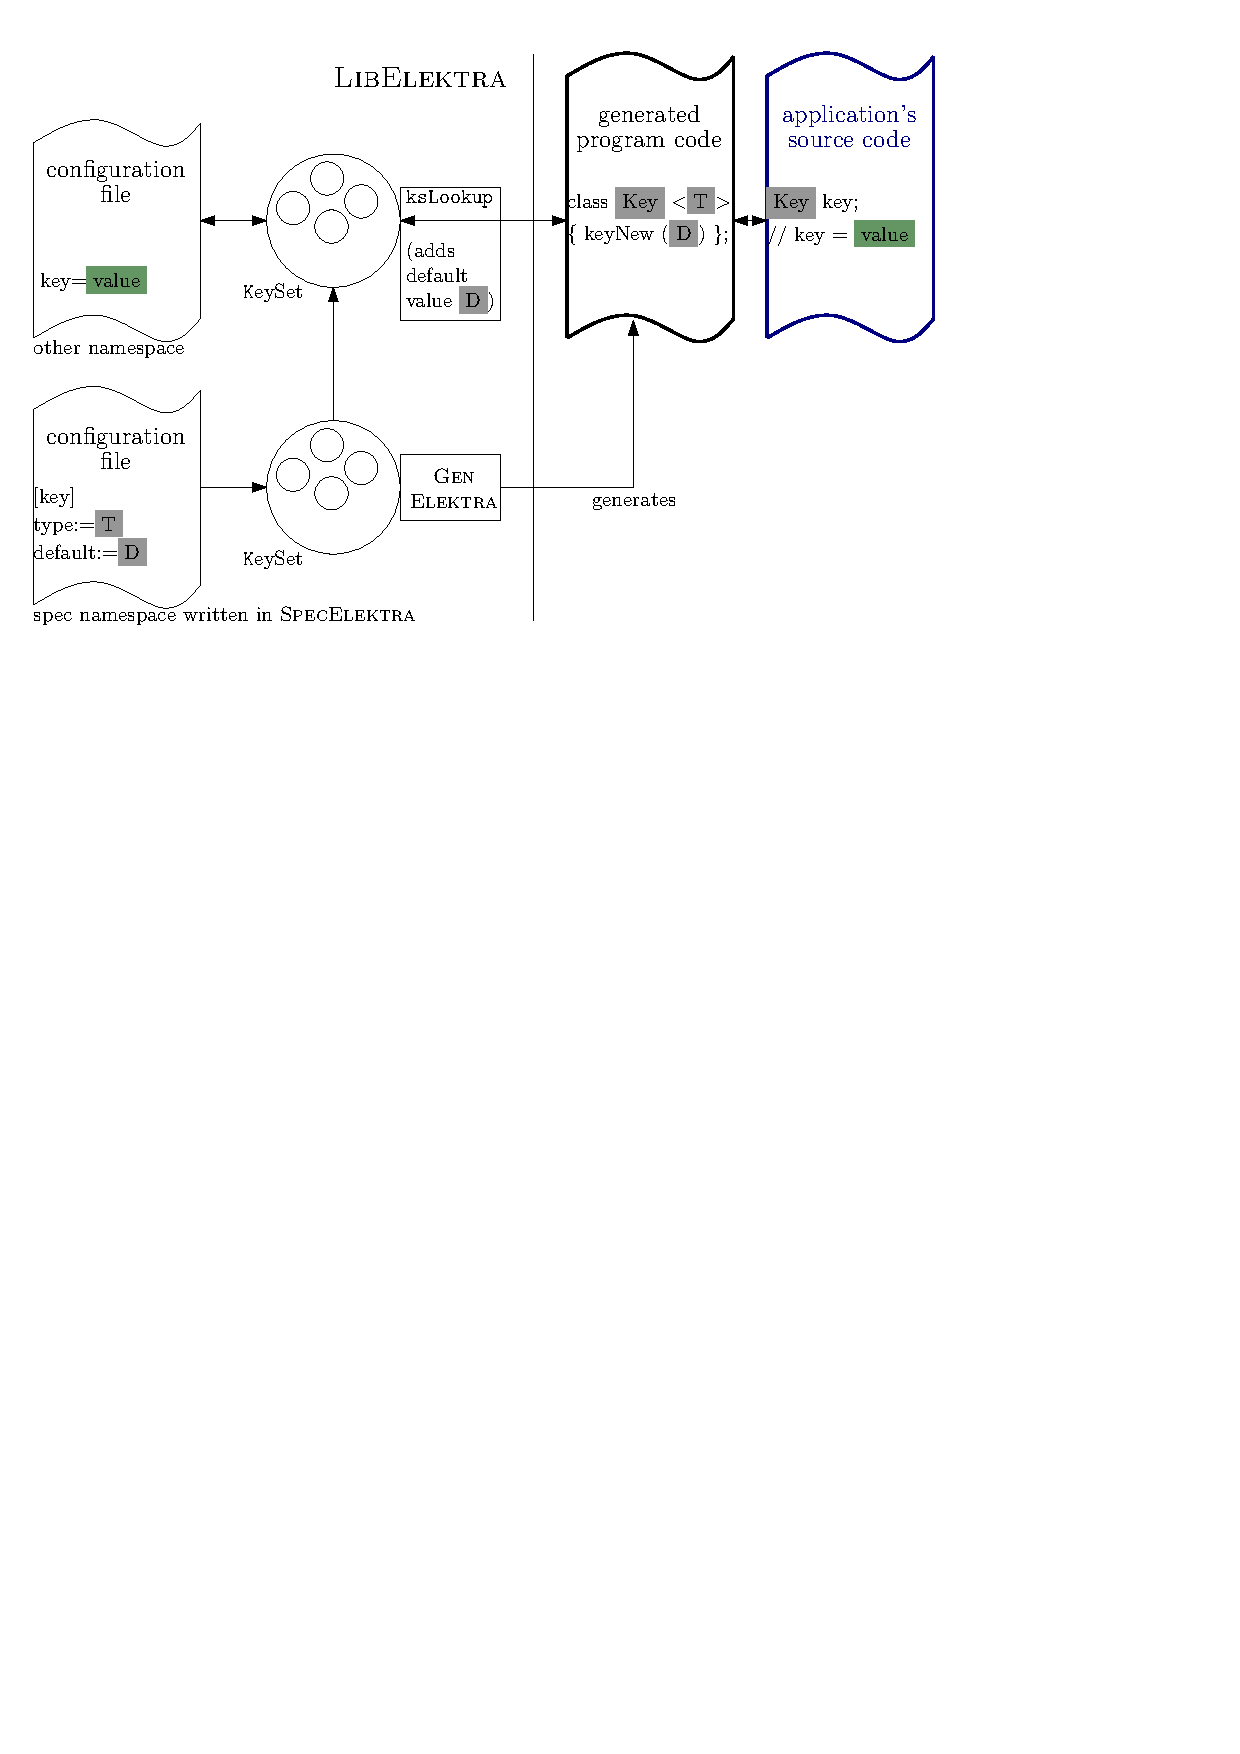
\includegraphics[scale=0.8]{flow}
\caption[Guarantees for configuration access.]{The guarantees for configuration access are given by \texttt{ksLookup}, although the specifications from generated source code might be used (if the configuration files are not available on the system).
Only the generated high-level frontend uses \texttt{ksLookup} but not the user's code.
The blue part needs to be supplied by the user.
The arrows indicate data flow of key sets.}
\label{fig:flow}
\end{figure}

\definecolor{shadecolor}{RGB}{150,150,150}
As we see in \figref{flow} the property \property{default} (grey box \colorbox{shadecolor}{{D}}) influences ^ksLookup^ (shown on the left side, implemented in \elektra{Lib}) and frontends (shown on the right side, generated by \elektra{Gen}).
Usually, the default value is dynamically read from a configuration file.
If the backend or configuration file is not available or is inconsistent, however, the hard-coded specification within the generated source code is used instead.
By comparing the built-in specification with the specification we got from the configuration file we can easily detect problems---such as missing default values.

The introduced operations on the key database (implemented in \elektra{Lib}) guarantee:
\begin{description}[font=\texttt]
\item[kdb.set:] to write only validated key sets into the key database (see \secref{kdb-api}).
Keys not adhering to the validation specification are rejected with an error.
\item[kdb.get:] to only return a validated key set.
Keys not adhering to the validation specification are dropped.\footnote{This only happens if \texttt{kdb.set} is bypassed.}
\end{description}

The code generator \elektra{Gen} guarantees for high-level APIs that:
\begin{itemize}
\item The configuration specifications are always available (see \secref{generated-apis}).
\item Only cascading lookups are used to look up contextual values.
\item For every generated contextual class the property \property{default} is present.
\end{itemize}

\begin{lemma}
When looking up keys in the high-level API, ^ksLookup^ never returns~$\NullKey$.
\end{lemma}

\begin{proof}
To be able to look up a key in the high-level API, by definition the property \property{default} must be present and a cascading lookup is used.
As we see in the algorithm ^ksLookup^ (\secref{lookup}), to use the property \property{default} three conditions need to be true:%
{\parfillskip=0pt plus .8\textwidth \emergencystretch=.5\textwidth \par}
\begin{description}[font=\normalfont\ttfamily]
\item[k == $\NullKey$:] can be false but then we already have a key and do not need the default.
\item[l \textbf{\color{BlueViolet}{is of namespace}} $\EmptyNameSpace$:] cannot be false because the code generator guarantees that only cascading lookups are used.
\item[specKey != $\NullKey$:] cannot be false, because the code generator ensures that the configuration specification is always present.
The ^specKey^'s presence (i.\,e., ^spec^ $\concatkey l$) is implied due to the presence of the property \property{default}.
\end{description}
\end{proof}

Default values are robust against context changes and reloading of configuration settings.
We are resistant against missing configuration settings:
Even if the backend cannot be used at all, we still have the specifications compiled in the application.

\begin{example}
We continue with \exref{introduction-solution} from page \pageref{ex:introduction-solution}:

\begin{code}[morekeywords={next}]
[slapd/threads/listener]
  check/range:=1,2,4,8,16
  context:=/slapd/threads/%cpu%/listener
  default:=1
  description:=One thread is adequate for up to 16 CPU cores.
  type:=long
\end{code}

Because of the presence of the property \property{default} the key \key{slapd/threads/listener} can be looked up safely.
The following values are tried in the given priority:
\begin{itemize}
\item Use the contextual value with the layer name ^cpu^ resolved in the backends.
After checking the specifications of the resulting key name, we look it up in any namespace:
\begin{itemize}
\item 
For 32 CPUs, the key name is \key{/slapd/threads/32/listener}.
\item 
If a specification for this configuration setting exist, it will be considered.
\item
Otherwise, we try all namespaces for \key{/slapd/threads/32/listener}.
\end{itemize}
\item Use the configuration setting ^/slapd/threads/listener^ in any namespace.
\item Otherwise, the lookup returns the default value ^1^.
\end{itemize}
\end{example}

